
\chapter{Spin one-half: Derivation of nonrelativistic Hamiltonian}

\section{Structure of the spin one-half theory}

The goal is to obtain a nonrelativistic theory from the relativistic.  To that end it'll help to have a clear understanding of the structure of the two theories.

\subsection{Relativistic framework for spin one-half}
In the relativistic theory, the electrons are part of a fermion field that also includes the positron anti-particle.  Since both are spin-1/2, each has two spin orientations.  There are, then, a total of four degrees of freedom. 

The relativistic Lagrangian for the fermion fields is
\beqa
\mathcal{L} &=&	
	\Psigbar(i \partial \cdot \gamma - e A \cdot \gamma - m)\Psig  - \frac{1}{4} F_{\mu\nu} F^{\mu\nu}.
\eeqa

The fermion fields are $\Psig$ ($\Psi$ being reserved for the fermion fields in the nonrelativistic theory), the photon field is $A$.   $m$ is the particle's mass, and $e$ the electron's charge.  The $\gamma$ matrices mix the different components.  %TODO better explanation of gamma matrices

It will be convenient to work in a representation which already suggests the nonrelativistic behavior.  At low momenta, it should be expected that the free electron and positron fields act approximately as independent fields.  This is exactly the case for the Dirac representation.   In the rest frame, a free particle can be said to be definitively an electron or positron, and in the Dirac representation these correspond to the upper and lower parts of the bispinor.  

In this representation, the gamma matrices are written
\beq
	\gamma^0 = \Mblock{1}{0}{0}{-1},
\eeq

\beq
	\gamma^i = \Mblock{0}{\sigma_i}{-\sigma_i}{0}.
\eeq	




The gamma matrices by themselves do not form a complete basis for this space.  To find such a basis products of the matrices can be considered.  It will make sense to consider combinations such that bilinears are Hermitian.  
 

There is the identity --- such bilinears transform as a scalar.

Symmetric combinations are not considered because $\{ \gamma^\mu, \gamma^\nu \}= g^{\mu\nu}$.  The antisymmetric combinations are explicitly
 \beqa
	  {[\gamma^0, \gamma^i]}
		&=&  2 \gamma^0 \gamma^i = \begin{pmatrix}	0 & 2\sigma_i \\ 2\sigma_i & 0\end{pmatrix},	\\
	  {[\gamma^i, \gamma^j ]}
		&=&	 \begin{pmatrix}	-2i\epsilon_{ijk}\sigma_k & 0 \\ 0 & -2i\epsilon_{ijk}\sigma_k\end{pmatrix}.
\eeqa
Using these a tensor like structure arises:
\beq
	\sigma^{\mu \nu} = i \frac{1}{2} [ \gamma^\mu, \gamma^\nu].	%defined as in Peskin p.50
\eeq

The specific form in the Dirac representation is
\beq
	\sigma^{ij} = \frac{i}{2} [ \gamma^i, \gamma^j] 
		= \epsilon_{ijk} \Mblock{\sigma_k}{0}{0}{\sigma_k},
\eeq
\beq
	\sigma^{0i} = i \gamma^0 \gamma^i 
			= \Mblock{0}{i \sigma_i}{i \sigma_i}{0}.
\eeq

The product of each gamma matrix in turn gives a pseudo-scalar:
\beq
	\gamma^5 = i \gamma^0 \gamma^1 \gamma^2 \gamma^3 = \Mblock{0}{1}{1}{0}.
\eeq
 
 The product of $\gamma^5$ and $\gamma^\mu$ gives a pseudo-vector
 \beq
 	\gamma^5 \gamma^\mu .
 \eeq
 
 
 
Solutions of the Dirac equation in momentum space are the spinors $\sr$.  They have four degrees of freedom, and can be treated as a bispinor consisting of an upper and lower spinor.  In the chiral basis the upper and lower components have opposite helicity; in the Dirac basis, opposite charge:
\beq
	\sr = \begin{pmatrix} \eta \\ \chi \end{pmatrix}.
\eeq



 
\subsection{Nonrelativistic framework for spin one-half}
The nonrelativistic theory describes a single particle, without its oppositely charged antiparticle.  
%FIXME a bit more word here


\beqa
	\eta &=& \left( 1  - \frac{\v{p}^2}{8m^2} \right ) w,	\\
	\chi &=& 	\frac{ \gv{\sigma} \cdot \v{p}}{2m} \left(1 - \frac{3\v{p}^2}{8m^2} \right ) w.	\\
\eeqa



 \section{Foldy-Wouthyusen approach}
 
The goal is to derive a nonrelativistic Hamiltonian or Lagrangian starting from relativistic theory.  (Having obtained one, we can easily obtain the other, of course.)  One method is to take the relativistic equations of motion and use them to obtain a Schrodinger like equation.

The starting point is the relativistic equations of motion, which can come from the Lagrangian of the relativistic theory.  Those equations can then be written in terms of the noncovariant quantities that appear in the nonrelativistic theory.  In doing so, the energy of the particle will now explicitly appear.

The relativistic theory will contain not only the particle of interest (the electron) but also its anti-particle (the positron.)  The nonrelativistic theory should contain only the electron.  Before obtaining an expression for the nonrelativistic Hamiltonian it will be necessary to somehow disentangle the two fields.  This is impossible in the general case, but as long as the energy and momenta in question are nonrelativistic, can be accomplished to any desired order.

Formally this is accomplished by the Foldy-Wouthyusen transformation, the result of which is that all operators are diagonal, the coupling between the particle and anti-particle suppressed to which ever order is desired.  However, practically the same result can be obtained by examining the normalisation of the two theory's particles.  By demanding that the Schrodinger like wave functions are appropriately normalized, the relationship between relativistic and nonrelativistic spinors can be established.

The result of this procedure will be an equation for the energy of the electron, accurate at some order in the nonrelativistic expansion.  However, it will not perfectly replicate the predictions of the high energy theory.  Unlike the process of NRQED, it does not truly incorporate the high energy sector of the theory.



\subsection{Equations of motion}

To reestablish the problem considered, the system to be examined is an electron placed in a loosely bound system with another charged particle, subject to an infinitesimal and constant magnetic field.  There will be, because of the bound system, an electric field acting on the electron as well as the external magnetic field.  When recoil effects are ignored, the electric field can just be taken as given.

The corrections to the gyromagnetic ratio of the electron are to be established.  There are two small scales that appear in the problem, the velocity $v$ of the electron and the infinitesimally small magnetic field $eB$.  The precision desired requires terms of up to order $mv^4$ and $ (e/m)Bv^2$.

The starting point will be the relativistic Lagrangian of Dirac.  However, remember that the technique to be used simply ignores behavior introduced by the high energy sector of the theory, even if it might effect the low energy behavior.  One such effect is corrections to the free gyromagnetic ratio of the electron, which first arise when one loop diagrams are considered.  Without such corrections the $g$-factor will be exactly $g=2$.

Knowing that there will actually be bound-state corrections proportional to $g-2$, it is necessary to somehow include this anomalous term.  The way to do so is to introduce a new local interaction into the Lagrangian, coming from the high energy radiative corrections which dress the electron vertex.  The Lagrangian to be used is, then
\beqa
\mathcal{L} &=&	
	\Psigbar(\cancel{D} - m)\Psi + \frac{1}{2} \mu' \bar{\Psi} \sigma^{\mu\nu}F_{\mu\nu} \Psig.
\eeqa
%TODO check \mu_0
$\mu'$ is the correction to the classical moment $\mu_0 = \frac{e}{2m}$, and is equal to $(g-2)/2 \mu_0$.  $D$ is the long derivative $\partial + ieA$.


From this Lagrangian the equations of motion of the particle may be obtained from the Euler-Lagrange method.  The Euler-Lagrange equation is
\beq
\pd{ \mathcal{L}}{{ \Psigbar } } - \partial_\mu \frac{\partial \mathcal{L}} {\partial (\partial_\mu { \Psigbar )} } 
	= 0	.
\eeq

In the Lagrangian above, we can consider that all differential operators act only on the right field $\Psi$.  (This freedom of choice comes from being able to rewrite the Lagrangian through integration by parts, without changing its physical meaning.)  So the second term in the Euler-Lagrange equation can be ignored, and after differentiating with respect to $\bar{\Psi}$ the following equation is obtained:
\beq
	(i\cancel{D} - m + \frac{1}{2} \mu'  \sigma^{\mu\nu}F_{\mu\nu} )\Psig = 0	.
\eeq
Writing explicitly in terms of the $\gamma$ matrices, this is
\beq \label{eq:Sh:eom}
	\left( (i\partial_\mu- eA_\mu)\gamma^\mu -m + i\mu' \frac{1}{4}[ \gamma^\mu, \gamma^\nu]F_{\mu\nu} \right) \Psig
		=0 .
\eeq
This equation of motion is invariant under Lorentz transformations.  It is written in terms of the Dirac bispinor $\Psi$, external fields $A_\mu$ and $F_{\mu\nu}$, and the gamma matrices.  To apply in to a nonrelativistic problem, the very first step will be to rewrite it in terms of the sorts of quantities that appear in that domain: three-vectors and scalars.

The scalars that appear will be $\partial_0= \partial_t$ and $A_0 = \Phi$.  The external fields $\v{E}$ and $\v{B}$ will appear explicitly, while the vector field $\v{A}$ will appear in the gauge-invariant operator $\gv{\pi} = \v{p} - e\v{A}$.  The gamma matrices can be written in terms of the Pauli spin matrices $\gv{\sigma}$.  Finally, the bispinor will be written in terms of its upper and lower components.

Of the terms that appear in \eqref{eq:Sh:eom}, all except the last are trivial to write in this manner.  To deal with that last term, the antisymmetric tensor $\sigma^{\mu\nu} =  \frac{1}{2}[\gamma^\mu, \gamma^\nu]$ needs to be written explicitly.

Using the antisymmetry of $\sigma^{\mu\nu} \equiv $, and that we deal with time-independent fields: %TODO fix sigma
\beqa
	F_{\mu\nu} \sigma^{\mu\nu} &=& F_{i}\sigma^{ij} - F_{0i}\sigma^{0i} 	- F_{i0}\sigma^{i0} +F_{00}\sigma^{00}	\\
		&=&	F_{ij} \sigma^{ij} -2F_{0i} \sigma^{0i}	\\
		&=&	2 \partial_i A_j \sigma^{ij} - 2\partial_i \Phi \sigma^{0i}	\\
		&=&	-2i \begin{pmatrix} \sigdot{B} & 0 \\ 0 & \sigdot{B}\end{pmatrix}	
			-2 \begin{pmatrix} 0 & \sigdot{E} \\ \sigdot{E} & 0 \end{pmatrix}.	
\eeqa

So far the discussion has been in position space.  To work out the nonrelativistic form it will be easier to talk about the equations of motion directly in terms of energy and momentum.  So replace $i\partial_t$ with $p_0$, and $i\partial_i$ with $p_i$.  Likewise, replace the gauge invariant derivative  $iD_i = \pi_i = p_i - eA_i$.

A solution of definite momentum $p$ to the equation is written in terms of upper and lower components
\beq
	u = \begin{pmatrix} \eta \\ \chi \end{pmatrix}.
\eeq


With these considerations, the \eqref{eq:Sh:eom} can be rewritten acting explicitly on the bispinor.
\scriptsize
\beq \label{eq:Sh:matrixEOM}
	\left\{
		\begin{pmatrix}
			p_0 - e\Phi	- m &	0	\\
			0	&	-p_0 + e\Phi - m	\\
		\end{pmatrix}
		+
		\begin{pmatrix}	0 & -\sigdotg{\pi} \\  \sigdotg{\pi} & 0 \end{pmatrix} 
		+\mu'\left [
			\begin{pmatrix}
				\sigdot{B} & 0 \\ 0 & \sigdot{B}
			\end{pmatrix}
			-i \begin{pmatrix}
				0 & \sigdot{E} \\ \sigdot{E} & 0
			\end{pmatrix}
		\right ] 
	\right\} \begin{pmatrix} \eta \\ \chi \end{pmatrix}
		= 0.
\eeq
\normalsize
This gives rise to exact coupled equations for $\eta$ and $\chi$.  So far this is in principle the same as the relativistic equation, only the form in which it is written is non covariant.

\subsection{Nonrelativistic limit}

The particle under consideration is a nonrelativistic electron.  Roughly, the expectation is that $\eta$ corresponds to the electron field and $\chi$ to that of the positron.  The off-diagonal terms in the equation above represent some sort of mixing between the electron and positron: the electron wave function still has some small positron component, that decreases as momentum is decreased.    The off diagonal component that does \emph{it} vanish at 0 momentum is proportional to $\mu'$, the term introduced to account for a high-energy process.

The upshot is that although the equation above is really a set of coupled equations for $\eta$ and $\chi$, $\chi$ will be small compared to $\eta$ --- the very leading order diagonal term will indicate that $\chi \sim \sigdotg{\pi} \eta$.

Because the off diagonal terms are small, the set of coupled equations may be solved perturbatively.  The particular quantity of interest is the nonrelativistic energy of the particle $\epsilon = p_0 - m$.  For a free particle, this would be
\beq
	\epsilon = p_0 - m \approx \frac{\v{p}^2}{2m} + \frac{\v{p}^4}{8m^3} + \mathcal{O}\left (\frac{\v{p}^6}{m^5} \right ).
\eeq  

In order to perform this perturbative analysis the order of various terms needs to be established.  It's evident that at leading order $\epsilon \sim mv^2$.  From earlier analysis,   $\Phi\sim mv^2$, $\v{\pi} \sim mv$, and $\v{E} \sim m^2v^3$.

First, find an expression for $\chi$ in terms of $\eta$.  The second of the set of equations represented by \eqref{eq:Sh:matrixEOM} is
\beq
	(-p_0 + e\Phi - m) \chi + \sigdotg{\pi} \eta + \mu'( \sigdot{B} \chi - i \sigdot{E}  \eta).
\eeq
Writing $p_0 = \epsilon + m$, and grouping terms, the result is that
\beq
	\left( \epsilon + 2m - \mu' \sigdot{B} \right ) \chi = \left( \sigdotg{\pi} - i\sigdot{E} \right) \eta	.
\eeq
It is necessary now to approximate $\chi$ in terms of $\eta$.  Because $\epsilon$ and $\abs{B}$ are smaller than $m$, and only second order terms are needed for the final result:
\beq
	\chi \approx	\frac{1}{2m} \left ( 1- \frac{\epsilon - e\Phi - \mu' \sigdot{B}}{2m} \right ) (\sigdotg{\pi} - i\mu' \sigdot{E} )\phi.
\eeq

With this expression $\chi$ may be eliminated from the first of the set of equations (at least at the necessary order).  The resulting equation will only involve $\eta$, and so may be used to solve for energy $\epsilon$ of  $\eta$.

The original equation is
\beq
	(p_0 - e\Phi - m) \eta - \sigdotg{\pi} \chi + \mu'( \sigdot{B}\eta  - i \sigdot{E} \chi ) .
\eeq
So again using $p_0 - m = \epsilon$
\beq
	\epsilon \eta 	= (e\Phi - \mu' \sigdot{B} )\eta + (\sigdot{E} + \sigdotg{\pi}) \chi	.
\eeq
Now the expression for $\chi$ in terms of $\eta$ may be used.
\beq
 	\epsilon \eta \approx (e\Phi - \mu' \sigdot{B} )\eta + (\sigdot{E} + \sigdotg{\pi})  \frac{1}{2m} \left ( 1- \frac{\epsilon - e\Phi - \mu' \sigdot{B}}{2m} \right ) (\sigdotg{\pi} - i\mu' \sigdot{E} )\eta .
\eeq				
 
Writing the $1/m$ and $1/m^2$ terms separately:
\beq
\begin{split}				\epsilon \eta		\approx& \left \{
		e\Phi - \mu' \sigdot{B} + \frac{ \exminus \explus}{2m}	\right. \\
		& \left. +\frac{1}{4m^2} \exminus (\mu' \sigdot{B} - [\epsilon - e\Phi]) \explus 	
	\right \} \eta	.
\end{split}
\eeq

Several of the terms are of too high order to consider.  A term with both $E$ and $B$, for instance, will be of higher order than $(e/m)\abs{B} v^2$.  Likewise, a term of $E \Phi$ or $E \epsilon$ is also too small.  Dropping all such:
\beq
	\epsilon \eta \approx \left \{
				e\Phi - \mu' \sigdot{B} + \frac{(\sigdotg{\pi})^2 - i\mu' [\sigdotg{\pi}, \sigdot{E}]}{2m}
				+\frac{1}{4m^2} \sigdotg{\pi} (\mu' \sigdot{B} - [\epsilon - e\Phi]) \sigdotg{\pi} 
			\right \} \eta.
\eeq
This is an expression for the energy $\epsilon$ of the particle, in terms of operators.  This will yield the nonrelativistic Hamiltonian.  There is still some manipulation required, though, because the right hand side also contains $\epsilon$.  But since the leading order terms don't, it may be perturbatively solved for.  (The above expression could be simplified somewhat, using the properties of $\sigma$ matrices for instance, but for now it is more convenient to write it compactly.)

To that end, the Hamiltonian can be split into leading order and second order terms.  The leading order will be of $mv^2$ and $(e/m)B$, while the next order will be suppressed by an additional factor of $v^2$.  Because the magnetic field is infinitesimally small no $B^2$ terms are needed. 
 Since the leading order term in H is $\mathcal{O}(mv^2)$, this suggests we split it into two parts: $H = H_0 + H_1 +\mathcal{O}(mv^6, (e/m) B v^4)$, where $H_1$ consists of only second order terms.
\beqa
	\hat{H_0} 
			&=&  e\Phi - \mu' \sigdot{B} + \frac{ (\sigdotg{\pi})^2}{2m},	\\
	\hat{H_1} 
			&=& -\frac{i\mu'}{2m}  [\sigdotg{\pi}, \sigdot{E}]
				+\frac{1}{4m^2} \sigdotg{\pi} (\mu' \sigdot{B} - [\epsilon - e\Phi]) \sigdotg{\pi} .
\eeqa
$H_1$ contains $\epsilon$, along with other terms of total order $mv^2$.  So to eliminate $\epsilon$ from $H_1$ it'll only be necessary to find it to leading order.
\beqa
	\epsilon \eta
			&=& \left(\hat{H_0} + \mathcal{O}(mv^4) \right)\eta 										\\
			&\approx& \left(e\Phi - \mu' \sigdot{B} + \frac{ (\sigdotg{\pi})^2}{2m}	\right) \eta.			
\eeqa
The operators on the right hand side, operating on $\eta$, produce $\epsilon$.  The combination actually needed is $\sigdotg{\pi} \epsilon \sigdotg{\pi}$.  To that end, start with $\sigdotg{\pi}^2 \epsilon$ and use commutation relations.
\beqa
	(\sigdotg{\pi})^2 (\epsilon - e\Phi) \eta		
			&=&	(\sigdotg{\pi})^2 \left ( \frac{(\sigdotg{\pi})^2}{2m}- \mu' \sigdot{B} \right )	\eta	\\
	\sigdotg{\pi} (\epsilon - e\Phi) \sigdotg{\pi}\eta
			&=&	\left( \frac{(\sigdotg{\pi})^4}{2m} 
				- \mu' (\sigdotg{\pi})^2 \sigdot{B} 
				- \sigdotg{\pi}[e\Phi, \sigdotg{\pi}]\right ) \eta
\eeqa
With this $\epsilon$ is eliminated, leaving:
\beq
	\hat{H}_1	=
		-\frac{i\mu'}{2m}  [\sigdotg{\pi}, \sigdot{E}]
		+\frac{1}{4m^2}\left(
			\mu' \sigdotg{\pi} \sigdot{B} \sigdotg{\pi}
			- \frac{(\sigdotg{\pi})^4}{2m} 
			+ \mu' (\sigdotg{\pi})^2 \sigdot{B} 
			+ \sigdotg{\pi}[e\Phi, \sigdotg{\pi}]
		\right).
\eeq
Some terms couple $A$ and $B$; they can be dropped.  Some simplification of the structures involving $\sigma$ matrices can be done.  To start with, simplify $(\sigdotg{\pi})^2$.
\beq
	(\sigdotg{\pi})^2 = \sigma_i \sigma_j \pi_i \pi_j = \pi^2 - i\epsilon_{ijk} \pi_i \pi_j \sigma_k.
\eeq
Since $\v{p} \times \v{p} = \v{A} \times \v{A} = 0$, from $\gv{\pi} \times \gv{\pi}$ only the cross terms survive:
\beq
	(\sigdotg{\pi})^2 = \pi^2 - i e \epsilon_{ijk}(p_i A_j - A_i p_j) = \pi^2 - e \sigdot{B}.
\eeq
Looking at the terms $\mu' \sigdotg{\pi} \sigdot{B} \sigdotg{\pi} + \mu' (\sigdotg{\pi})^2 \sigdot{B}$, they contain an anticommutator involving $B$ and $p$.  Because the magnetic field is assumed to be constant, $p$ and $B$ commute, so: 
\beqa
\{ \sigdot{B}, \sigdot{p} \}	&=&		B_i p_j \{\sigma_i, \sigma_j\}	\\
		&=&	2\v{B}\cdot \v{p}.
\eeqa
The commutator of $\Phi$ and a derivative operator should give the electric field $E$:
\beq
	[ \Phi, \sigdotg{\pi} ]	= [ \Phi, p_i] \sigma_i = -iE_i \sigma_i = -i\sigdot{E} .
\eeq
Using these identities, the Hamiltonian can be expressed as:
\beq
	\hat{H_0} 
			=  e\Phi - \mu' \sigdot{B} + \frac{ \pi^2}{2m} - \frac{e}{2m} \sigdot{B},	\\
\eeq
\beq
	\hat{H}_1	=
		- \frac{\pi^4}{8m^3}  
		+ e\frac{p^2}{4m^3} \sigdot{B}
		-i \frac{\sigdotg{\pi} \sigdot{E}}{4m^2} 
		+ \mu' \left(	
			\frac{ \sigdot{p} \v{B}\cdot \v{p} }{2m^2}
			-\frac{i[\sigdotg{\pi}, \sigdot{E}]}{2m} 
		\right ).
\eeq
There are still some simplifications that can be made to terms quadratic in $\sigma$, but it'll be more convenient for now to keep $H$ written as is.

\subsection{Foldy-Wouthyusen Transform}

To find a complete description of a single nonrelativistic particle in normal quantum mechanics, we must work in a basis where the lower component $\chi$ is truly negligible, at least at the desired order.  While there exists a formal technique for finding this Foldy-Wouthyusen transformation, for our purposes we can simply demand that the wave function after transformation $\phis = (1 + \Delta)\eta$ obeys $\langle \phis, \phis \rangle = 1$.  This follows from the necessity of probability conservation.

To find the necessary transformation, we can use the relativistic current density, and demand it equal that of the nonrelativistic Schrodinger-like wave functions.   Using the expression for $\chi$ in terms of $\eta$:
\beqa
	\int d^3x (\eta^\dagger \eta + \chi^\dagger \chi) 	
		&=& \int d^3x 	\left[ \eta^\dagger \phi + \left (\frac{\sigdotg{\pi}}{2m} \phi \right)^\dagger
										   \left (\frac{\sigdotg{\pi}}{2m} \eta \right)
						\right ]	\\
		&=& \int d^3x 	\eta^\dagger \left[ 1 + \frac{ (\sigdotg{\pi})^2 }{4m^2} \right ] \eta.
\eeqa
Since we know that $\langle \phis, \phis \rangle=1$ this shows that if $\eta = \left( 1 - \frac{ (\sigdotg{\pi})^2 }{8m^2} \right )\phis$, the current conservation works out correctly.


We now need to find the form of $\hat{H}$ after this transformation.  For now work with the general form:
\beq
	\epsilon \eta = (\hat{H}_0 + \hat{H}_1) \eta .
\eeq
After changing to the Schrodinger like wave functions, this becomes:
\beq
	\epsilon \left (1 - \frac{(\sigdotg{\pi})^2}{8m^2} \right )\phi_S 
		=  (\hat{H}_0 + \hat{H}_1) \left(1 - \frac{(\sigdotg{\pi})^2}{8m^2}\right)\phi_S .
\eeq
To the order needed the inverse of $1 + \sigdotg{\pi}^2 / 8m^2 $ is just $1 - \sigdotg{\pi}^2 / 8m^2 $, so eliminating that on the left hand side gives:
\beq
	\epsilon \phi_S =  (1 + \frac{(\sigdotg{\pi})^2}{8m^2})(\hat{H}_0 + \hat{H}_1) (1 - \frac{(\sigdotg{\pi})^2}{8m^2})\phi_S .
\eeq
Since $H_1$ is already second order, these further corrections don't involve it directly.  Expressing the result as a commutator:
\beq
	\epsilon \phi_S = \left (  \hat{H}_0 + \frac{1}{8m^2}[(\sigdotg{\pi})^2, \hat{H}_0] + \hat{H}_1 \right )\phi_S .
\eeq
So under the FW transformation, the leading order term is unchanged, and the second order term is:
\beq
	 \hat{H}_1 \to \hat{H}_1' = \hat{H}_1 + \frac{1}{8m^2}[(\sigdotg{\pi})^2, \hat{H}_0] .
\eeq

The final step is to simplify the commutator $ [(\sigdotg{\pi})^2, \hat{H}_0] $.
  
\beq [(\sigdotg{\pi})^2, \hat{H}_0] = [(\sigdotg{\pi})^2, e\Phi - \mu' \sigdot{B} + \frac {(\sigdotg{\pi})^2}{2m}] . \eeq

Obviously $(\sigdotg{\pi})^2$ commutes with itself, so that term vanishes.  Since $\sigdot{B}$ is constant, that commutator will also disappear.  Writing $\sigdotg{\pi}$ as shown earlier:
$$[(\sigdotg{\pi})^2, \mu' \sigdot{B}] =[\pi^2 - e \sigdot{B}, \mu'\sigdot{B}] = 0 .$$


The non-trivial part is the commutation of the derivative operators with the electric potential $\Phi$. 
\beqa
[(\sigdotg{\pi})^2, \hat{H}_0] &=& [(\sigdotg{\pi})^2, e\Phi] \\
		&=&	e( \sigdotg{\pi}[\sigdotg{\pi},  \Phi] + [\sigdotg{\pi},  \Phi]\sigdotg{\pi}) \\
		&=&	i e( \sigdotg{\pi} \sigdot{E} + \sigdot{E} \sigdotg{\pi} ). \\
\eeqa
So, writing down the new $H_1'$:
\beqa
\hat{H}_1' 
	&=&  \hat{H}_1 + \frac{i e}{8m^2}( \sigdotg{\pi} \sigdot{E} + \sigdot{E} \sigdotg{\pi} )	\\
	&=&	 -\frac{\pi^4}{8m^3} + e \frac{p^2}{4m^3}\sigdot{B} - \frac{ie}{8m^2}[\sigdot{E},\sigdotg{\pi}]
		 + \mu' \left( \frac{ (\sigdot{p}) (B \cdot p) }{2m^2} - \frac{i}{2m}[\sigdot{E},\sigdotg{\pi}] \right).
\eeqa

\subsection*{Nonrelativistic Hamiltonian}
From the relativistic equations of motion, a nonrelativistic Hamiltonian was defined in terms of Schrodinger-like wave functions that conserve probability.  The final result may now be written down.  For comparison with other work, rather than writing in terms of $\mu'$, it will be written in terms of the gyromagnetic ratio $g$.  Because terms proportional to $g-2$ may enter separately, it is convenient to express all $g$ dependent terms as linear combinations of $g$ and $g-2$. 

So the entire Hamiltonian, using $\mu' = \frac{g-2}{2}\mu_0 = \frac{g-2}{2}\frac{e}{2m} $, is:
\beqa
H	&=&	e\Phi  + \frac{ \pi^2}{2m} 
		- \frac{\pi^4}{8m^3} 
		- (1 + \frac{g-2}{2})\frac{e}{2m} \sigdot{B}	
		+ e \frac{p^2}{4m^3}\sigdot{B}
\\&&  	+ \frac{ie}{8m^2}(1 + (g-2))[\sigdot{E},\sigdotg{\pi}]
		+ (g-2) \frac{e}{2m}  \frac{ (\sigdot{p}) (\v{B} \cdot \v{p}) }{4m^2}  	\\
&=&		e\Phi  + \frac{ \pi^2}{2m}
		-\frac{\pi^4}{8m^3} 
		- \frac{e}{2m} \Big\{
			\frac{g}{2}\sigdot{B} - \frac{p^2}{2m^2}\sigdot{B}
\\&&		- (g-2) \frac{ (\sigdot{p}) (\v{B} \cdot \v{p}) }{4m^2} 
			+(g-1) \gv{\sigma} \cdot (\v{E} \times \gv{\pi})
		\Big \}	
\\&=&
		e\Phi  + \frac{ \pi^2}{2m} -\frac{\pi^4}{8m^3} 
		- \frac{e}{2m} \Big\{
			\frac{g}{2} \left( 1 - \frac{p^2}{2m^2} \right) \sigdot{B} + \frac{g-2}{2} \frac{p^2}{2m^2}\sigdot{B}
	\\&&		- \frac{g-2}{2} \frac{ (\sigdot{p}) (\v	{B} \cdot \v{p}) }{2m^2} 
			+\left(\frac{g}{2} + \frac{g-2}{2}\right) \gv{\sigma} \cdot (\v{E} \times \gv{\pi})
		\Big \}	.
\eeqa
			


 
 
 

%skeleton of calculation
\section{Effective Lagrangian approach}
%define spinors and structures
Instead of starting from the relativistic equations of motion and rewriting them in the form of a Schrodinger like equation, the method of NRQED can be employed.  The nonrelativistic Lagrangian can be written in the most general way, but ignoring all possible terms that will have too small a contribution to calculations.  The coefficients before each term will be unknown, but there is a straightforward method of fixing them.

Within the realm of NRQEDs validity, it should produce the same predictions as QED.  The same physical process can be calculated in both frameworks, and then the results compared.  The calculation in QED will then fix the coefficients in NRQED.  In comparing the two calculations it will be necessary to write the QED results nonrelativisitcally, in the same manner as was done for the equation of motion.
%TODO mention free vs. nonfree spinors?

For spin one-half, up to the order desired, the form of the NRQED Lagrangian involving two fermion fields has been derived in the previous chapter.  It is
\beq \label{eq:Sh:nrL-2f}
\begin{split}
\mathcal{L}_{NRQED} = & \fnrb \Bigg\{
		iD_0 +  \frac{\v{D}^2}{2m}  + 	\frac{\v{D}^4}{8m^2}
		 + c_F \frac{e}{m} \v{S} \cdot \v{B}
		+ c_D \frac{e (\v{D} \cdot \v{E} - \v{E} \cdot \v{D})}{8m^2} 
\\	& + c_S \frac{ i e \v{S} \cdot(\v{D} \times \v{E} - \v{E} \times \v{D}}{8m^2}
		+ c_{W1} \frac{ e \v{D}^2 \v{S} \cdot \v{B} + \v{S} \cdot \v{B} \v{D}^2 }{8m^3}
		- c_{W2} \frac{e D_i (\v{S} \cdot \v{B}) D_i}{4m^3}
\\	&		+c_{p'p} \frac{ e [ (\v{S}\cdot \v{D})(\v{B} \cdot \v{D}) + (\v{B} \cdot \v{D})(\v{S}\cdot \v{D})]}{8m^3}
		\Bigg \} \fnr.
\end{split}
\eeq
Each term contains two fermion fields, and zero, one or two powers of the photon field.  Terms with a different number of photon fields, of course, correspond to different physical processes.  But because gauge invariance is a necessary feature of the theory, the coefficients of many terms involving the photon field are constrained to be the same as that of terms with a smaller number of such fields.  For instance, the gauge invariant term $\v{D}^2/(2m)$ is: 
\beq	
	\frac{\v{D}^2}{2m} = \frac{ \grad^2 - i e (\grad \cdot \v{A} + e \v{A} \cdot \grad ) - e^2 \v{A}^2 }{2m}.
\eeq
The first term above, containing $\grad^2$, is a purely kinetic term.  The other two represent interactions with one or two photon fields.  To fix these coefficients, two physical processes could be calculated and compared with the QED results, but in the end they must have the same coefficient as guaranteed by gauge invariance.

Obviously not every term goes this same way.  The term with $\v{S} \cdot \v{B}$, for instance, is in and of itself gauge-invariant, and so there is no option but to calculate it from a process involving a single photon.  For the necessary terms appearing in the above Lagrangian, it would suffice to consider just the one photon processes.  However, since in principle some of the interesting coefficients could be calculated from two photon diagrams, this also will be done. 

To fix these terms, some physical process must be chosen.  For the one photon terms, scattering off an external field will be calculated.  For the two photon terms, Compton scattering will be used.

\section{Electron scattering off an external field in QED}
%First form
To fix all the terms in the NRQED Lagrangian which have a single power of the photon field, it suffices to calculate the scattering of an electron off an external field, as represented (in QED) by the diagram

\begin{center}   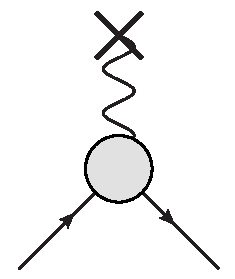
\includegraphics[scale=0.8]{eps/blob-wave} \end{center} 
	%TODO add additional diagrams


The leading order contributions (in QED) to this interaction come from the fundamental electron vertex.  There are radiative corrections to this process, starting at the one loop order.  In principle, such calculations (up to some desired order in $\alpha$) should be included in the QED calculation.  

However, it turns out that the actual \emph{form} of the interaction is highly constrained by the symmetries of the theory.  No matter the source of contributions to the vertex, their effects can be incorporated into two coefficients or form factors.  The NRQED coefficients can then be written in terms of these form factors, which can later be calculated to whatever precision is necessary.  

The first symmetry that constrains the interaction is that it must be invariant under Lorentz transformations.  Since every term involves the photon field $A_\mu$ and has external fermion legs, then the interaction must be proportional to the general form:
\beq
	A_\mu \srb(p') \Gamma^\mu(p', p) \sr(p).
\eeq 	
and $\srb(p') \Gamma^\mu(p', p) \sr(p) $ must transform as a Lorentz vector.  If it did not, the whole would not be Lorentz invariant.  To leading order $\Gamma^\mu = \gamma^\mu$, since the fundamental vertex is just that.  The corrections, whatever the exact details of the processes which produce them, can only depend on the momenta $p$ and $p'$, in addition to constants $m$ and $e$, and such structures as may act upon the spinors.

A basis for such structures is known, with well defined Lorentz transformations.  That gives scalar, vector, tensor, pseudo-vector, and pseudoscalar terms.  From the momenta in the problem can be constructed scalar and vector quantities.  What symmetries control the allowed terms?

In addition to proper Lorentz invariance, it is necessary that the interaction as a whole preserve parity.  Since $A$ is a vector, the term $\srb \Gamma^\mu \sr$ must also behave as a vector under parity transformations.  And there is no Lorentz invariant combination of external momenta that can be written that is not even under parity.   Because of this, there can be no contribution from the pseudovector and pseudoscalar bilinears.

The vector bilinear $\srb \gamma^\mu \sr$ already has the correct transformation properties.  From the scalar bilinear $\srb \sr$, a vector can be constructed by adjoining a single power of the momentum.  (As, for example, $p^\mu \srb \sr$.)  And after contracting one index of the tensor with a momentum vector, it will also behave as a vector.

The momenta terms available are $p$ and $p'$.  However, the terms constructed from them are not independent, because each must separately obey current conservation.  So whatever terms go into $\Gamma^\mu$, $q_\mu \srb \Gamma^\mu \sr = 0$.  The unique scalar term will be
\beq
	\frac{p^\mu + p'^\mu}{2m} \srb \sr,
\eeq     
which vanishes because $(p'+p) \cdot (p'-p) = p'^2 - p^2 = m^2- m^2=0$.

The unique tensor term allowed will be
\beq
	\frac{q_\nu}{2m} \srb \sigma^{\mu\nu} \sr,
\eeq
which conserves current because $\sigma^{\mu\nu}$ is antisymmetric.  So from these considerations, the general form of the vertex will have three terms, each with a momentum dependant coefficient:
\beq \label{eq:Sh:Gamma}
	\srb \Gamma^\mu \sr 
		= 	c_1(p, p') \frac{p^\mu + p'^\mu}{2m} \srb \sr
			+ c_2(p, p') \srb \gamma^\mu \sr
			+ c_3(p, p') \frac{q_\mu}{2m} \srb \sigma^{\mu\nu} \sr.
\eeq

However, there is one more consideration.  From the Dirac equation can be derived the Gordon identity, which relates these three terms:
\beq \label{eq:Sh:gordon}
	\srb \gamma^\mu \sr = \srb \left( \frac{p^\mu + p'^\mu }{2m} + \frac{i \sigma^{\mu\nu}q_\nu}{2m} \right ) \sr.
\eeq

With this, any one of the terms in \eqref{eq:Sh:Gamma} can be rewritten as some combination of the other two, and its coefficient effectively absorbed into the other two.  To write down the most general form of the vertex, one need only choose two of the three terms.  Which two to choose might depend on the nature of the calculation; at any rate, there are always three paths to go down.

In the calculation of scattering off an external field an agnostic approach will be taken at first.  The scattering amplitude is some combination of the three bilinears.  The goal is to rewrite the scattering amplitude in nonrelativistic language.  So, each bilinear in turn will be rewritten in this manner.

The vertex can be written in each of three ways.  The form factors will be defined with respect to the particular combination of $\gamma^\mu$ and $\sigma^{\mu\nu}$ terms.

\beq
	\Gamma^\mu = \gamma^\mu F_1(q^2) + i \frac{\sigma^{\mu\nu}q_\nu}{2m} F_2 (q^2).
\eeq

Using the Gordon identity to write this in terms of the scalar and vector bilinears, the result is
\beq
	\Gamma^\mu = \gamma^\mu [F_1(q^2) + F_2(q^2) ]  -  \frac{p^\mu  + p'^\mu }{2m}F_2 (q^2).
\eeq

And writing in terms of the scalar and tensor:
\beq
	\Gamma^\mu = \frac{p^\mu  + p'^\mu }{2m} F_1(q^2) + i \frac{\sigma^{\mu\nu}q_\nu}{2m} [F_1(q^2) + F_2(q^2) ] .
\eeq

%TODO move this section up a bit?
The momentum dependence can be uniquely written in terms of $q^2$.  The factors must be Lorentz invariant, so only such combinations of momenta can be considered.  From the momenta $p$ and $p'$, only three such quantities can be constructed.  But since the external fermions are on mass-shell, $p^2 = p'^2 = m^2$.  That leaves only $p \cdot p' = m^2 + p \cdot q$, and this can be related to $q^2$ by noting that since $p^2 = p'^2$,
\beq
	p^2 = p^2 + 2p\cdot q + q^2  \to q^2 = -\frac{1}{2} p \cdot q.
\eeq


Given that there exist these three ways to write the vertex, there are three ways to perform the calculation.  The scattering amplitude will have the form
\beq	
	i M = 	A_\mu \srb(p') \Gamma^\mu(p', p) \sr(p),
\eeq
and no matter which way $\Gamma^\mu$ is written, a nonrelativistic expansion in terms of $\phis$ will be needed.  For now an agnostic approach will be taken, and the expressions for each of the three possible bilinears found.


\subsection{Nonrelativistic expressions for the bilinears}
To compare with the NRQED scattering amplitude, everything needs to be written with consistent language.  We start with the relativistic bilinears, each of which behaves like a four vector, and appears in the amplitude dotted with the external field $A$.  Any dot products $a \cdot b$ should instead be written as $a_0 b_0 - \v{a} \cdot \v{b}$.  To this end, it might be necessary to treat the spatial and time-like components of the four-vector bilinears separately.

The bispinors $u$ will be first written in terms of upper and lower components $\eta$, $\chi$, and then in terms of the nonrelativistic wave spinors $w$.  The relationship between the two sets are
\begin{eqnarray}
	\label{eq:Sh:eta-w} \eta(p) &=& \left( 1 - \frac{\v{p}^2}{8m^2} \right ) \wx(p),	\\
	\label{eq:Sh:chi-w}  \chi(p)	&=& \frac{ \sigdot{p} }{2m} \left(1  - \frac{3\v{p}^2}{8m^2} \right ) \wx(p).
\end{eqnarray}
In writing in terms of the upper and lower components,  the explicit expressions of the $\gamma$ matrices, as well as $\sigma^{\mu\nu}$ will be needed.  

Of course the above expressions for the spinors in terms of $w$ is approximate.  In the NRQED Lagrangian, the terms we wish to fix involve $A_0$ with up to two powers of momentum (such as $\grad \cdot \v{E}$), and $A_i$ with up to three (as in $\sigdot{B} \v{p}^2$).  Because only the case of a constant magnetic field is needed, in any term which will explicitly contain $B$ higher derivatives may be ignored.  Throwing away unneeded terms, whatever is left can be used to calculate the scattering amplitude and compare with NRQED.

This same general procedure will be followed for each of the bilinears.

\subsubsection{Terms involving the scalar bilinear}
Start with the first bilinear, a scalar coupled with a momentum four-vector.  Rewrite it in terms of $\eta$ and $\chi$.
\beq
	(p + p')^\mu \srb \sr  = (p + p')^\mu \left( \eta^\dagger \eta - \chi^\dagger \chi \right ).
\eeq
Now express in terms of $\wx$, replacing $\eta$ and $\chi$ according to \eqref{eq:Sh:eta-w} and \eqref{eq:Sh:chi-w}.
\beq
	(p + p')^\mu \srb \sr = (p + p')^\mu \left \{
		\wxd \left( 1 - \frac{ \v{p'}^2}{8m^2} \right )  \left( 1 - \frac{ \v{p}^2}{8m^2} \right ) \wx
		- \wxd \left( \frac{ \gv{\sigma} \cdot \v{p'}}{2m} \frac{ \gv{\sigma} \cdot \v{p}}{2m} \right ) \wx \right \}.
\eeq 
Combining the terms, and dropping terms beyond the order needed:
\beq
	(p + p')^\mu \srb \sr = (p + p')^\mu \wxd \left( 
		1 -  \frac{ \v{p}^2 + \v{p'}^2}{8m^2} - \frac{ \gv{\sigma} \cdot \v{p'} \gv{\sigma} \cdot \v{p} }{4m^2} 
		\right ) \wx.
\eeq
The term quadratic in $\sigma$ can be simplified, using $\sigdot{p'} \sigdot{p} = \v{p} \cdot \v{p'} + i\gv{\sigma} \cdot \v{q} \times \v{p}$.
\beq \label{eq:Sh:Si}
	(p + p')^\mu \srb \sr  = (p + p')^\mu \wxd \left( 
		1 -  \frac{ \v{p}^2  +2 \v{p} \cdot \v{p'} +  \v{p'}}{8m^2} - \frac{i\gv{\sigma} \cdot \v{q} \times \v{p} }{4m^2} 
		\right ) \wx.
\eeq

The spatial part is straightforward, but the time-like part is 
\beq
	(p + p')^0 \srb \sr  = (p + p')_0 \wxd \left( 
		1 -  \frac{ \v{p}^2  +2 \v{p} \cdot \v{p'} +  \v{p'}^2 }{8m^2} - \frac{i\gv{\sigma} \cdot \v{q} \times \v{p} }{4m^2} 
		\right ) \wx.
\eeq
Approximating the relativistic energies gives $p_0 = m + \v{p}^2 / (2m) $.  So
\beq
	p_0 + p'_0 \approx 2m + \frac{ \v{p}^2 + \v{p'}^2 }{2m} = 2m\left( 1 +  \frac{ \v{p}^2 + \v{p'}^2 }{4m^2} \right ).
\eeq
Then using this correction to the leading order term gives the time like component:
\beq
	(p + p')^0 \srb \sr  = 2m  \wxd \left( 
		1 +  \frac{ \v{p}^2   - 2 \v{p} \cdot \v{p'} +  \v{p'} }{8m^2} - \frac{i\gv{\sigma} \cdot \v{q} \times \v{p} }{4m^2} 
		\right ) \wx,
\eeq
\beq \label{eq:Sh:S0}
	(p + p')^0 \srb \sr  \approx 2m  \wxd \left( 
		1 +  \frac{ \v{q}^2 }{8m^2} - \frac{i\gv{\sigma} \cdot \v{q} \times \v{p} }{4m^2} 
		\right ) \wx.
\eeq




\subsubsection{Terms involving the vector bilinear}
For the term $\srb \gamma^\mu \sr$ it'll be necessary to treat the spatial/time-like indices separately, since they have different spinor structure.

The time-like part is:
\beq
	\srb \gamma^0 u = u^\dagger u,
\eeq
which in terms of $\eta$ and $\chi$ is just
\beq
	= \eta^\dagger \eta + \chi^\dagger \chi.
\eeq
Then rewritten with $\wx$
\beq
	= 	\wxd \left( 1 - \frac{ \v{p'}^2}{8m^2} \right )  \left( 1 - \frac{ \v{p}^2}{8m^2} \right ) \wx
		+ \wxd \left( \frac{ \gv{\sigma} \cdot \v{p'}}{2m} \frac{ \gv{\sigma} \cdot \v{p}}{2m} \right ) \wx 
\eeq
Which is, at the order needed
\beq
	=	 \wxd \left( 
		1 -  \frac{ \v{p}^2 + \v{p'}^2}{8m^2} + \frac{ \gv{\sigma} \cdot \v{p'} \gv{\sigma} \cdot \v{p} }{4m^2} 
		\right ) \wx.
\eeq
Simplifying the last term, using $\sigma_i \sigma_j = \delta_{ij} + i\epsilon_{ijk}\sigma_k$, gives
\beq \label{eq:Sh:V0}
	\srb \gamma^0 \sr = 
			\wxd \left( 
		1 -  \frac{ \v{q}^2 }{8m^2} + \frac{i \gv{\sigma} \cdot \v{q} \times \v{p} }{4m^2} 
		\right ) \wx.
\eeq





The spatial part is
\beq
	\srb \gamma^i \sr = \sr^\dagger \gamma^0 \gamma^i \sr.
\eeq
Writing the matrices explicitly,
\beq
	 \srb^\dagger \begin{pmatrix}
		0 & \sigma_i \\ \sigma_i & 0 		
	\end{pmatrix} \sr,
\eeq
which in terms of spinors is
\beq
	 \eta^\dagger \sigma_i \chi + \chi^\dagger \sigma_i \eta.
\eeq
Replacing the spinors with $w$ gives
\beq
	 \wxd \left\{
		\left( 1 - \frac{ \v{p'}^2}{8m^2}   \right ) \frac{ \sigma_i \sigdot{p} }{2m} \left( 1 - \frac{3\v{p}^2}{8m^2} \right )
			+ \left( 1 - \frac{ 3\v{p'}^2}{8m^2} \right )  \frac{  \sigdot{p'} \sigma_i }{2m} \left( 1 - \frac{\v{p}^2}{8m^2} \right )
	\right\} \wx.
\eeq
Using $\v{p'}^2 = \v{p}^2$ gives
\beq
	= \wxd \left\{
		\frac{ \sigma_i \sigdot{p}  + \sigdot{p'} \sigma_i }{2m} \left( 1 -\frac{ \v{p}^2}{2m^2} \right )
	\right\} \wx.
\eeq
Then $\sigma_i \sigma_j = \delta_{ij} + i\epsilon_{ijk} \sigma_k$
\beq
	= \wxd \left\{
		\frac{ p_i + \epsilon_{ijk} p_j \sigma_k + p'_i  + \epsilon_{jik} p'_j \sigma_k }{2m} \left( 1 -\frac{ \v{p}^2}{2m^2} \right )
	\right\} \wx.
\eeq
So finally
\beq \label{eq:Sh:Vi}
	\srb \gamma^i \sr  = \wxd \left\{
		\frac{ p_i + p'_i - \epsilon_{ijk} q_j \sigma_k }{2m} \left( 1 -\frac{ \v{p}^2}{2m^2} \right )
	\right\} \wx
\eeq



\subsubsection{Terms involving the tensor bilinear}
The tensor term is subject to an additional simplification.  Because the process under considering is elastic scattering off an external static field, terms involving $q_0$ can be dropped.  Under this approximation $q_\nu \sigma^{\mu\nu} \approx  q_j \sigma^{\mu j}$.

Dealing first with the case where $\mu=i$, write the tensor structure explicitly as a matrix:  
\beq
	\srb  \frac{i}{2m} q_j \sigma^{ij} \sr 
		=  \frac{i \epsilon_{ijk} q_j}{2m} \srb \Mblock{\sigma_k}{0}{0}{\sigma_k} \sr.
\eeq
Write in terms of spinors this is
\beq
	 \frac{i \epsilon_{ijk} q_j}{2m} \left( \eta^\dagger \sigma_k \eta - \chi^\dagger \sigma_k \chi \right ),
\eeq
and then in terms of $\wx$
\beq
	= \frac{i \epsilon_{ijk} q_j}{2m} \wxd \left \{
		\left( 1 - \frac{\v{p'}^2}{8m^2} \right ) \sigma_k \left( 1 - \frac{\v{p'}^2}{8m^2} \right )- \frac{ \gv{\sigma} \cdot \v{p'} \sigma_k \gv{\sigma} \cdot \v{p} }{4m^2} \wx
	\right \}.
\eeq
There now appears a term with a triple product of $\sigma$ matrices.  That can be simplified with the following expression:
\beq
	\sigma_a \sigma_b \sigma_c = \sigma_a (\delta_{bc} + i\epsilon_{bcd}\sigma_d)
		=	\sigma_a \delta_{bc} - \sigma_b \delta_{ca} + \sigma_c \delta_{ab} + i \epsilon_{abc}.
\eeq
Using that identity, 
\beq
	\srb  \frac{i}{2m} q_j \sigma^{ij} \sr 
		= \frac{i \epsilon_{ijk} q_j}{2m} \wxd \left \{
			\sigma_k \left( 1 - \frac{\v{p'}^2  + \v{p}^2}{8m^2} \right ) - \frac{ \gv{\sigma} \cdot (\v{p} + \v{p'})p_k - \sigma_k \v{p} \cdot \v{p'} + i \epsilon_{akc} q_a p_c }{4m^2} 
		\right \} \wx .
\eeq

This can be further simplified by combining the like terms $\sigma_k (\v{p'}^2 + \v{p}^2 ) - 2 \sigma_k \v{p} \cdot \v{p'} = \sigma_k \v{q}^2$.
\beq
	\srb  \frac{i}{2m} q_j \sigma^{ij} \sr 
		= \frac{i \epsilon_{ijk} q_j}{2m} \wxd \left \{
			\sigma_k \left( 1 - \frac{\v{q}^2}{8m^2} \right ) - \frac{ \gv{\sigma} \cdot (\v{p} + \v{p'})p_k + i \epsilon_{akc} q_a p_c }{4m^2} 
		\right \} \wx .
\eeq
Now it is necessary to consider exactly what derivatives of the field $A_i$ are to be kept.  The assumption is that $B$ is constant and so $\partial_i B_j = 0$.  Contracted with $A_i$ above, $\epsilon_{ijk} A_i q_j \sim B_k$.  So besides the leading factor, no terms with $q$ are needed.  Applying this simplification,
\beq \label{eq:Sh:Ti}
	\srb  \frac{i}{2m} q_j \sigma^{ij} \sr 
		= \frac{i \epsilon_{ijk} q_j}{2m} \wxd \left \{
			\sigma_k - \frac{ \gv{\sigma} \cdot \v{p} p_k  }{2m^2} 
		\right \} \wx.
\eeq






The case with $\mu=0$ goes as follows.
\beq
	\srb  \frac{i}{2m} q_j \sigma^{0j} \sr
		=	 - \frac{q_j}{2m} \srb \gamma^0 \gamma^j \sr 		
 		=  - \frac{q_j}{2m} \sr^\dagger \gamma^j \sr.
\eeq
Explicitly in matrix form 
\beq
	\srb  \frac{i}{2m} q_j \sigma^{0j} \sr  = - \frac{q_j}{2m} \sr^\dagger \Mblock{0}{\sigma_j}{\sigma_j}{0} \sr. 
\eeq
 Written in terms of spinors, and Galilean three-vector $q^j= -q_j$.
 \beq
 	\srb  \frac{i}{2m} q_j \sigma^{0j} \sr = \frac{q^j}{2m}  \left( \eta^\dagger \sigma_j \chi - \chi^\dagger \sigma_j \eta \right ).
 \eeq
 And then in terms of $w$:
\beq
	=  \frac{q^j}{2m}  \wxd \left \{
		\left(1 - \frac{\v{p'}^2}{8m^2} \right )  \frac{ \sigma_j \gv{\sigma} \cdot \v{p} }{2m} \left(1 - \frac{3\v{p}^2}{8m^2} \right )
		- \left(1 - \frac{3 \v{p'}^2}{8m^2} \right ) \frac{\gv{\sigma} \cdot \v{p'} \sigma_j  }{2m} \left(1 - \frac{\v{p}^2}{8m^2} \right )
	\right \} \wx.
\eeq

This bilinear is contracted with $A_0$, and so actually, only terms involving two additional powers of momenta need be kept.
\beq
	\srb  \frac{i}{2m} q_j \sigma^{0j} \sr =  \frac{q^j}{2m}  \wxd \left \{
		  \frac{ \sigma_j \gv{\sigma} \cdot \v{p} }{2m} 
		-  \frac{\gv{\sigma} \cdot \v{p'} \sigma_j  }{2m} 
	\right \} \wx,
\eeq
or simplifying using the commutator of $\sigma$ matrices
\beq 
	\srb  \frac{i}{2m} q_j \sigma^{0j} \sr =   \frac{q^j}{2m}  \wxd \left \{
		\frac{ 2 i\epsilon_{jik} p_i \sigma_k  - q_i - i\epsilon_{ijk} q_j \sigma_k }{2m} 
	\right \} \wx.
\eeq
One term above vanishes because of symmetry
\beq \label{eq:Sh:T0}
\srb  \frac{i}{2m} q_j \sigma^{0j} \sr
	=  -  \wxd \left \{
			\frac{  \v{q}^2  }{4m^2} 
			- \frac{  i\gv{\sigma} \cdot \v{q} \times \v{p}   }{2m^2} 
	\right \} \wx.
\eeq


\subsubsection{Contraction of bilinears with $A_0$}
The scattering amplitude is composed of bilinears coupled to the field $A$.  The transferred momentum $\v{q}$ becomes a derivative of this field, $\v{q} \to -i\grad$ or equivalently $\grad \to i\v{q}$.  Before finally writing down the full vertex, the coupling of $A$ and the bilinears should be worked out, including appropriate transformations involving $\v{q}$.

First consider terms with $A_0(q)$.  The relation between $\v{q}$ and $\v{E}$ is that $\v{E} = - \grad A_0 = i\v{q} A_0$.  Terms quadratic in $q$ give $\v{q}^2 A_0 = -\grad^2 A_0 =  \grad \cdot \v{E}$.


The term with $A_0$ coupled with the scalar bilinear \eqref{eq:Sh:S0} gives
\beqaL  \label{eq:Sh:SA0}
	eA_0  (p + p')^0 \srb \sr &\approx&
		eA_0 \wxd \left( 
		1 +  \frac{ \v{q}^2 }{8m^2} - \frac{i\gv{\sigma} \cdot \v{q} \times \v{p} }{4m^2} 
		\right ) \wx	\\
	& \approx &
			 \wxd \left( 
				eA_0  +  \frac{ e \grad \cdot \v{E} }{8m^2} - \frac{e \gv{\sigma} \cdot \v{E} \times \v{p} }{4m^2} 
				\right ) \wx.
\eeqaL
The term involving the vector bilinear term \eqref{eq:Sh:V0} is
\beqaL    \label{eq:Sh:VA0}
	eA_0 \srb \gamma^0 u &=& 
			eA_0 \wxd \left( 
		1 -  \frac{ \v{q}^2 }{8m^2} + \frac{i \gv{\sigma} \cdot \v{q} \times \v{p} }{4m^2} 
		\right ) \wx	\\
	&=& 
		 \wxd \left( 
		eA_0  - \frac{ e \grad \cdot \v{E} }{8m^2} + \frac{ e\gv{\sigma} \cdot \v{E} \times \v{p} }{4m^2} 
		\right ) \wx.
\eeqaL

The third type of term, with the tensor bilinear appearing:
\beqaL  \label{eq:Sh:TA0}
e A_0 \srb  \frac{i}{2m} q_j \sigma^{0j} \sr
	&=&  - e A_0 \wxd\left \{
			\frac{  \v{q}^2  }{4m^2} 
			- \frac{  i\gv{\sigma} \cdot \v{q} \times \v{p}   }{2m^2} 
	\right \} \wx	\\
	&=&  -   \wxd \left \{
			\frac{e  \grad \cdot \v{E} }{4m^2} - \frac{e \gv{\sigma} \cdot \v{E} \times \v{p} }{2m^2} 
	\right \} \wx.
\eeqaL

\subsubsection{Contraction of bilinears with $A_i$}

Terms with $\v{A}$ and $\v{q}$ give rise to terms with $\v{B} = \grad \times \v{A}$.  There are some that are simple to transform, containing $\epsilon_{ijk} iq_i A_j \to B_k$.  In others, the way $B$ arises is less clear.  

Consider the expression $(\v{p} + \v{p'})\cdot \v{A}  (\gv{\sigma} \cdot \v{p} \times i\v{q})$.  Kinematic constraints will help in expressing this term.  First, it is convenient to develop an identity for $iq_i (\v{p} + \v{p'}) \cdot \v{A}$.  Using $\epsilon_{ijk} B_k = i(q_i A_j - q_j A_i)$:
\beq
	(p + p')_i \epsilon_{ijk} B_k = (p + p')_i  \left( i q_i A_j - i q_j A_i \right ).
\eeq
There are additional conditions coming from the fact that this is elastic scattering.  Since in this case $ ( \v{p'} + \v{p}) \cdot \v{q} = \v{p'}^2 - \v{p}^2 = 0$, the $(p+p')_i q_i$ term vanishes, leaving
\beq
	(p + p')_i \epsilon_{ijk} B_k = -i (p + p')_i q_j A_i = -i q_j(\v{p} + \v{p'}) \cdot \v{A} .
\eeq

This gives the identity
\beq \label{eq:Sh:pqA}
i q_j (\v{p} + \v{p'}) \cdot \v{A}  =  - \epsilon_{ijk} (p + p')_i  B_k.
\eeq
This identity helps reduce the more complicated term:
\beqa
(\v{p} + \v{p'}) \cdot \v{A} ( \gv{\sigma} \cdot \v{p} \times i\v{q} )
	&=&	 \sigma_i p_j  \epsilon_{ijk} [i q_k (\v{p} + \v{p'}) \cdot \v{A} ]	\\
	&=&	- \sigma_i p_j \epsilon_{ijk} [ \epsilon_{\ell k m} (p + p')_\ell B_ m]	\\
	&=&	 \sigma_i p_j \epsilon_{ijk} [ \epsilon_{\ell m k} (p + p')_\ell B_ m]	\\
	&=&	\sigma_i p_j (p+p')_\ell B_m [\delta_{i \ell} \delta_{jm} - \delta_{i m} \delta_{j \ell}]	\\
	&=&	\gv{\sigma} \cdot  (\v{p} + \v{p'}) \v{B} \cdot \v{p} - \gv{\sigma} \cdot \v{B} (\v{p} + \v{p'}) \cdot \v{p}.
\eeqa
For the case of a constant $\v{B}$, any terms of the type $q_i B_j$ vanish.  So the above reduces to
\beq \label{eq:Sh:A-p-id}
(\v{p} + \v{p'}) \cdot \v{A}  (\gv{\sigma} \cdot \v{p} \times i\v{q} )
	= 2 \{  (\gv{\sigma} \cdot  \v{p})( \v{B} \cdot \v{p}) - \v{p}^2 \gv{\sigma} \cdot \v{B} \}.
\eeq

Now consider $A_i$ coupled with each of the particular bilinear expressions.  (Remember that here $A_i = -\v{A}_i$.)  With the term involving a scalar bilinear \eqref{eq:Sh:Si}
\beqaL \label{eq:Sh:SAi}
	\frac{A_i (p + p')^i}{2m} \srb \sr  &=& - \frac{\v{A} \cdot (\v{p} + \v{p'} ) }{2m} \wxd \left( 
		1 -  \frac{ \v{p}^2  +2 \v{p} \cdot \v{p'} +  \v{p'}}{8m^2} - \frac{i\gv{\sigma} \cdot \v{q} \times \v{p} }{4m^2} 
		\right ) \wx	\\
	 &=&	- \wxd  \left [ \frac{e \v{A} \cdot (\v{p} + \v{p'} ) }{2m} \left(1 - \frac{\v{p}^2}{4m^2} \right )  \right ] \wx
	- \wxd  \left [  \frac{ 	 e (\gv{\sigma} \cdot  \v{p})( \v{B} \cdot \v{p}) - e \v{p}^2 \gv{\sigma} \cdot \v{B} }{4m^2} \right ] \wx . \nonumber
\eeqaL
The term involving a vector bilinear coupled to $A_i$ comes from \eqref{eq:Sh:Vi}
\beqaL \label{eq:Sh:VAi}
A_i \srb \gamma^i \sr  &=& \wxd \left\{
		A_i \frac{ p_i + p'_i - \epsilon_{ijk} q_j \sigma_k }{2m} \left( 1 -\frac{ \v{p}^2}{2m^2} \right )
	\right\} \wx \\
	&=&- \wxd \left \{
		 \frac{ \v{A} \cdot (\v{p} + \v{p'}) + \gv{\sigma} \cdot \v{B} }{2m} \left(1 - \frac{\v{p}}{2m^2} \right ) 
	\right\} \wx.
\eeqaL
Finally the term with a tensor gives
\beqaL  \label{eq:Sh:TAi}
	A_i \srb  \frac{i}{2m} q_j \sigma^{ij} \sr 
		&=& \frac{i \epsilon_{ijk} A_i q_j}{2m} \wxd \left \{
			\sigma_k - \frac{ \gv{\sigma} \cdot \v{p} p_k  }{2m^2} 
		\right \} \wx \\ 
		&=&  - \wxd \left \{ 
				\frac{ \gv{\sigma} \cdot \v{B} }{2m} - \frac{ (\gv{\sigma} \cdot \v{p}) (\v{B} \cdot \v{p}) }{4m^2}
			\right \} \wx.
\eeqaL

% Start of comparison
\subsubsection{Full vertex}

Now that the three bilinears have been calculated, the complete scattering amplitude can be written down.  Each of the three forms should prove equivalent.  To simplify comparison, the coupling to $A_0$ and $A_i$ can be treated separately.

The first has $	\Gamma^\mu = \gamma^\mu F_1(q^2) + i \frac{\sigma^{\mu\nu}q_\nu}{2m} F_2 (q^2)$.  Using \eqref{eq:Sh:VA0} and \eqref{eq:Sh:TA0}
\beq
	eA_0 \srb  \Gamma^0 \sr = 
		 F_1   \wxd \left( 
		eA_0  - \frac{ e \grad \cdot \v{E} }{8m^2} + \frac{ e\gv{\sigma} \cdot \v{E} \times \v{p} }{4m^2} 
		\right ) \wx
		- F_2    \wxd \left \{
			\frac{e  \grad \cdot \v{E} }{4m^2} - \frac{e \gv{\sigma} \cdot \v{E} \times \v{p} }{2m^2} 
	\right \} \wx.
\eeq
The second is	$\Gamma^\mu = \gamma^\mu [F_1(q^2) + F_2(q^2) ]  -  \frac{p^\mu  + p'^\mu }{2m}F_2 (q^2)$.  Using \eqref{eq:Sh:VA0} and \eqref{eq:Sh:SA0}.
\beq
	eA_0 \srb  \Gamma^0 \sr = 
		 (F_1 + F_2)  \wxd \left( 
		eA_0  - \frac{ e \grad \cdot \v{E} }{8m^2} + \frac{ e\gv{\sigma} \cdot \v{E} \times \v{p} }{4m^2} 
		\right ) \wx
		- F_2   \wxd \left( 
		eA_0  +  \frac{ e \grad \cdot \v{E} }{8m^2} - \frac{e \gv{\sigma} \cdot \v{E} \times \v{p} }{4m^2} 
		\right ) \wx.
\eeq
The third combination is $	\Gamma^\mu = \frac{p^\mu  + p'^\mu }{2m} F_1(q^2) + i \frac{\sigma^{\mu\nu}q_\nu}{2m} [F_1(q^2) + F_2(q^2) ] $.  Using \eqref{eq:Sh:SA0} and \eqref{eq:Sh:TA0}
\beq
	 A_0 \srb  \Gamma^0 \sr = 
		F_1 \wxd \left( 
		eA_0  +  \frac{ e \grad \cdot \v{E} }{8m^2} - \frac{e \gv{\sigma} \cdot \v{E} \times \v{p} }{4m^2} 
		\right ) \wx
		- [F_1 + F_2] \wxd \left \{
			\frac{e  \grad \cdot \v{E} }{4m^2} - \frac{e \gv{\sigma} \cdot \v{E} \times \v{p} }{2m^2} 
	\right \} \wx.
\eeq
Taking any of these three results and collecting like terms gives the result
\beq
		 A_0 \srb  \Gamma^0 \sr = \wxd \left(  
			F_1  eA_0
			+ [F_1 + 2 F_2] \left [ 
				\frac{e \gv{\sigma} \cdot \v{E} \times \v{p} }{4m^2}  - \frac{e  \grad \cdot \v{E} }{8m^2}
			\right ]
		\right ) \wx,
\eeq
so the calculations are consistent with the Gordon identity.

Now turning to the coupling with $\v{A}$.  The first has $	\Gamma^\mu = \gamma^\mu F_1(q^2) + i \frac{\sigma^{\mu\nu}q_\nu}{2m} F_2 (q^2)$.  Using \eqref{eq:Sh:VAi} and \eqref{eq:Sh:TAi}
\beq
\begin{split}
	e A_i \srb \Gamma^i \sr = & 
		 - e F_1 \wxd \left \{
		 \frac{ \v{A} \cdot (\v{p} + \v{p'}) + \gv{\sigma} \cdot \v{B} }{2m} \left(1 - \frac{\v{p}}{2m^2} \right ) 
	\right\} \wx
	\\& - e F_2  \wxd \left \{ \frac{ \gv{\sigma} \cdot \v{B} }{2m} - \frac{ (\gv{\sigma} \cdot \v{p}) (\v{B} \cdot \v{p}) }{4m^2}
			\right \} \wx.
\end{split}
\eeq
The second is	$\Gamma^\mu = \gamma^\mu [F_1(q^2) + F_2(q^2) ]  -  \frac{p^\mu  + p'^\mu }{2m}F_2 (q^2)$.  Using \eqref{eq:Sh:VAi} and \eqref{eq:Sh:SAi}:
\beq \begin{split}
	e A_i \srb \Gamma^i \sr = & 
		- e [F_1 + F_2] \wxd \left \{
		 \frac{  \v{A} \cdot (\v{p} + \v{p'}) +  \gv{\sigma} \cdot \v{B} }{2m} \left(1 - \frac{\v{p}}{2m^2} \right ) 
	\right\} \wx
	\\& + e F_2 \wxd  \left [ \frac{e \v{A} \cdot (\v{p} + \v{p'} ) }{2m} \left(1 - \frac{\v{p}^2}{4m^2} \right )  \right ] \wx
	+ eF_2 \wxd  \left [  \frac{ 	 e (\gv{\sigma} \cdot  \v{p})( \v{B} \cdot \v{p}) - e \v{p}^2 \gv{\sigma} \cdot \v{B} }{4m^2} \right ] \wx.
\end{split} \eeq
The third combination is $\Gamma^\mu = \frac{p^\mu  + p'^\mu }{2m} F_1(q^2) + i \frac{\sigma^{\mu\nu}q_\nu}{2m} [F_1(q^2) + F_2(q^2) ] $.  Using \eqref{eq:Sh:SAi} and \eqref{eq:Sh:TAi}
\beq \begin{split}
	e A_i \srb \Gamma^i \sr = & 
		 e F_1 \wxd  \left [ \frac{e \v{A} \cdot (\v{p} + \v{p'} ) }{2m} \left(1 - \frac{\v{p}^2}{4m^2} \right )  \right ] \wx
		 + e F_1 \wxd  \left [  \frac{ (\gv{\sigma} \cdot  \v{p})( \v{B} \cdot \v{p}) - e \v{p}^2 \gv{\sigma} \cdot \v{B} }{4m^2} \right ] \wx
	\\&	-[F_1 + F_2] \wxd \left \{ \frac{ \gv{\sigma} \cdot \v{B} }{2m} - \frac{ (\gv{\sigma} \cdot \v{p}) (\v{B} \cdot \v{p}) }{4m^2}
			\right \} \wx.
\end{split} \eeq

For any of these paths, the total result is that
\beq \begin{split}
	e A_i \srb \Gamma^i \sr =  \wxd \Bigg \{
		- \frac{ e\v{A} \cdot (\v{p} + \v{p'} ) }{2m} \left( 1 - \frac{\v{p}^2}{2m^2} \right )
		- [F_1 + F_2] \frac{ e \gv{\sigma} \cdot \v{B} }{2m} 
	\\	+ F_1 \frac{ e \gv{\sigma} \cdot \v{B} \v{p}^2 }{4m^3} 
		+ F_2 \frac{ (\gv{\sigma} \cdot \v{p}) (\v{B} \cdot \v{p}) }{4m^2}
	\Bigg \} \wx.
\end{split}
\eeq

\section{Electron scattering off an external field in NRQED}
Earlier, the Lagrangian \eqref{eq:nr:L-half} for spin one-half particles was calculated.  To calculate the scattering off an external field in this theory, only those terms that include one power of the electromagnetic field are needed.  Call that part of the Lagrangian containing such terms $\mathcal{L}_A$.  This set of terms need not, by themselves, be gauge invariant.  However, previously care was taken to group terms in a gauge invariant way.  So first the terms of $\mathcal{L}_A$ must be disentangled from the gauge invariant terms (involving one or more powers of $\v{D}$).



First take the kinetic terms, involving simple powers of $\v{D}$.  $\v{D} = \grad - ie\v{A}$, so
\beq
	\v{D}^2 = (\nabla_i - ieA_i)(\nabla_i - ieA_i).
\eeq
It is a mixture of terms with two, one, or no powers of the external field $A$.  If just the terms with one power of $\v{A}$ are included, what remains is
\beq
	-ie( A_i \nabla_i + A_i \nabla_i = -ie \{A_i, \nabla_i\}.
\eeq
So from $\v{D}^2/ 2m$ emerges, in $\mathcal{L}_A$,  $-ie \{\nabla_i, A_i\}/2m$ in  $\mathcal{L}_A$.

The second kinetic term is $\v{D}^4$:
\beq
	\v{D}^4 = (\nabla_i - ieA_i)(\nabla_i - ieA_i) (\nabla_j - ieA_j)(\nabla_j - ieA_j),
\eeq
or
\beq
	\v{D}^4 = ( \grad^2 - ie \{A_i, \nabla_i\} - e^2 \v{A}^2)( \grad^2 - ie \{A_j, \nabla_j\} - e^2 \v{A}^2).
\eeq
Keeping again only the terms with a single power of $A$, what remains may be expressed as the double anti-commutator
\beq
	-ie \{ \grad^2, \{\nabla_i, A_i \} \} .
\eeq

There are then several terms involving one or more powers of $D$ combined with either $E$ or $B$.  Since only terms with a single power of the field are of interest, in all such terms $\v{D}$ may be replaced with $\grad$.



So finally, writing all such terms from the original Lagrangian involved in scattering off an external field leaves:
\small
\beq 
\label{eq:Sh:nrL-A}
\begin{split} 
\mathcal{L}_A = \fnrb \Bigg (  -eA_0 
		&- ie  \frac{ \{\nabla_i, A_i \} }{2m} -ie \frac{ \{\grad^2, \{\nabla_i, A_i \}  \} }{8m^3} 
		+ c_F e \frac{\v{S} \smalldot \v{B}} {2m}   	
		+ c_D \frac{ e(\v{\grad} \smalldot \v{E} - \v{E} \smalldot \v{\grad} ) }{8m^2}	
			\\&	+ c^{1}_S \frac{ ie \v{S} \smalldot ( \v{\grad} \times \v{E} - \v{E} \times \v{\grad} )}{8m^2}
		+ c_{W_1} \frac{ e [ \v{\grad}^2 (\v{S} \smalldot \v{B} ) + (\v{S} \smalldot \v{B} ) \v{\grad}^2] }{8m^3}	
		\\& - c_{W_2} \frac{ e \nabla^i (\v{S} \smalldot \v{B} ) \nabla^i }{4m^3}
		+ c_{p'p} \frac{ e [ (\v{S} \smalldot \v{\grad}) (\v{B} \smalldot \v{\grad}) + (\v{B} \smalldot \v{\grad})(\v{S} \smalldot \v{\grad}) }{8m^3} \Bigg )\fnr.
\end{split} \eeq
\normalsize



\subsubsection{Calculation of one photon scattering}



The form Lagrangian that will account for all interactions with a single photon is now established.  From this, the idea is to calculate a particular process: scattering off an external field, with incoming momentum $\v{p}$, outgoing $\v{p'}$, and $\v{q} = \v{p'} - \v{p}$. 
One diagram could be associated with each term in \eqref{eq:Sh:nrL-A}, but the total amplitude is just going to be the sum of all these one-photon vertices.  These of course can just be read off directly from the Lagrangian.

It is necessary to switch to the language of momentum space.  The recipe is this: replace the fields $\Psi$ with the spinors $\phi$, and any operator $\grad$ acting will become $i\v{p}$ if it acts on the right, $i\v{p'}$ if it is to the left.

The terms originating from $D^2$ are:
\beq
	- ie  \frac{ \{\nabla_i, A_i \} }{2m} ,
\eeq
which in position space become
\beq
	e \frac{ \v{A} \cdot (\v{p} + \v{p'}) }{2m}.
\eeq

While the terms arising from $D^4$
\beq
-ie \frac{ \{\grad^2, \{\nabla_i, A_i \}  \} }{8m^3} ,
\eeq
become
\beq
- e \frac{ \v{A} \cdot (\v{p} + \v{p'}) (\v{p'}^2 + \v{p}^2 ) }{8m^3} .
\eeq


Some of the expressions involving $\grad$ and $\v{E}$ can be simplified.  Because $E_i = -\partial_i \Phi$
\beq
	\v{\grad} \times \v{E} - \v{E} \times \v{\grad} =  - 2 \v{E} \times \v{\grad}.
\eeq
And also
\beq
\v{\grad} \smalldot \v{E} - \v{E} \smalldot \v{\grad} = (\partial_i E_i).
\eeq


After all these considerations, the total scattering amplitude off an external field may be written down, before any assumptions are applied:



 \mbox{
\begin{minipage}{1.0in}
   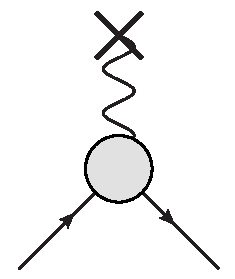
\includegraphics[scale=0.5]{eps/blob-wave} 
\end{minipage}
=
\begin{minipage}{1.6in}
\scriptsize
\beq
\begin{split}
	 ie\wnrb \Bigg(& - A_0 +    \frac{ \v{A} \cdot (\v{p} + \v{p'}) }{2m} 
		- \frac{  \v{A} \cdot (\v{p} + \v{p'}) \v{p}^2 + \v{p'}^2 \v{A} \cdot (\v{p} + \v{p'}) }{8m^3} 
	\\&	+ c_F  \frac{\v{S} \smalldot \v{B}} {2m}   	
		+ c_D \frac{ ( \partial_i E_i ) }{8m^2}	
		+ c^{1}_S \frac{  \v{E} \times \v{p} }{4m^2}
		- c_{W_1}  \frac{  (\v{S} \smalldot \v{B} ) (\v{p}^2 + \v{p'}^2)  }{8m^3}
	\\&	+ c_{W_2} \frac{  (\v{S} \smalldot \v{B} ) (\v{p} \cdot \v{p'}) }{4m^3}
		-  c_{p'p} \frac{  (\v{S} \smalldot \v{p'}) (\v{B} \smalldot \v{p}) + (\v{B} \smalldot \v{p'}) (\v{S} \smalldot \v{p}) }{8m^3} \Bigg )\wnr .
\end{split}
\eeq 

\end{minipage}
}



This can be simplified somewhat.  Choose the gauge such that $\nabla_i A_i = 0$.  If elastic scattering is specified, then kinematics dictate that $\v{p'}^2 = \v{p}^2$.   Finally, if $\v{B}$ is constant, the $c_W$ terms become indistinguishable, since $[ \nabla_i, B_j] = 0$.    (It is only this last assumption that costs any information, since it becomes impossible to determine $c_{W_1}$ and $c_{W_2}$ separately. )  Then the scattering amplitude, as calculated from $\mathcal{L}_{NRQED}$, is:

\beq 
\begin{split} \label{eq:Sh:nrqedScatter}
	iM =&
		ie\wnrb \Bigg(  -A_0 +  \frac{ \v{A} \cdot \v{p} }{m} - \frac{  (\v{A} \cdot \v{p}) \v{p}^2   }{2m^3} 
		+ c_F  \frac{\v{S} \smalldot \v{B}} {2m}   	
		+ c_D \frac{ ( \partial_i E_i ) }{8m^2}	
		\\&	+ c^{1}_S \frac{  \v{E} \times \v{p} }{4m^2}
		- (c_{W_1} -c_{W_2}) \frac{   (\v{S} \smalldot \v{B} ) \v{p}^2  }{4m^3}	
		-  c_{p'p} \frac{   (\v{S} \smalldot \v{p}) (\v{B} \smalldot \v{p})  }{4m^3} \Bigg )\wnr .
\end{split}
\eeq




\section{Compton scattering in QED}
The relevant terms in the NRQED Lagrangian can all be fixed by the previous calculation of scattering off an external field, because even though there are terms involving two powers of the photon field, the requirement of gauge invariance means they share a coefficient with one photon terms.  However, for reasons of self consistency it would be good to check that the coefficients really do work out the same if calculated independently.

The easiest process to calculate involving two photons will be Compton scattering.   

\section{The two-photon vertex of NRQED}
%TODO cleanup notation
In the NRQED Lagrangian, in addition to the terms involving the fermions interaction with a single photon, there are terms which represent the interaction of a fermion with two photons.  At the order needed, all such terms are fixed by gauge invariance.  There are terms, such as those involving $\v{E}^2$, that would are by themselves gauge invariant, but these occur at too high an order.  (The order of such a term would be $E^2 / m^3 \sim mv^6$.)

So though the coefficients of concern are all fixed by considering just the one-photon interactions, they could also be fixed from considering two-photon interactions.  Since it \emph{is} possible, it makes sense to do so, as a check of consistency.  In this section, the coefficients of two-photon terms in the NRQED Lagrangian will be fixed from QED calculations.

As before, this will involve calculating some physical process in both QED and NRQED, and comparing the result.  The simplest two photon process to consider is Compton scattering.  By calculating Compton scattering in each theory, the coefficients desired will be obtained.

This is not quite as straightforward as in the case of the one-photon scattering, for the following reason: while the one-photon scattering is a local interaction in both QED and NRQED, Compton scattering will involve some mix of local and non-local diagrams.  In QED, there are of course no local interactions between a fermion and two photons.  The situation is most readily stated diagrammatically.

In QED, the leading order diagrams contributing to Compton scattering are:

\vspace{1em}
 \mbox{
\begin{minipage}{1in}
   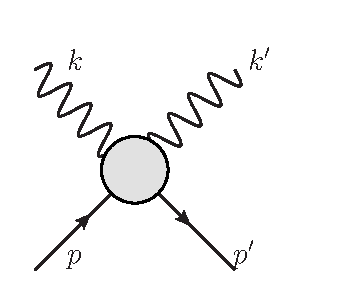
\includegraphics[scale=0.5]{eps/2photon-blob} 
\end{minipage}
$	=	\hspace{1em} 	 $
\begin{minipage}{1.5in}
   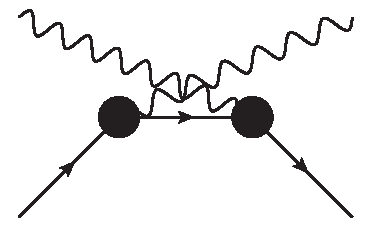
\includegraphics[scale=0.5]{eps/Tree-crossed}
\end{minipage}
$\hspace{1em}   +  \hspace{1em} $
\begin{minipage}{1.5in}
   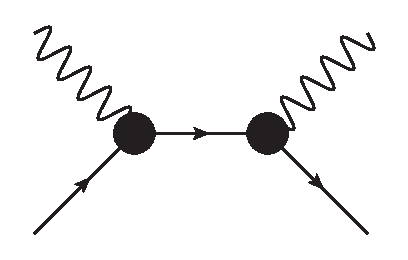
\includegraphics[scale=0.5]{eps/Tree-uncrossed} 
\end{minipage}
} 
\vspace{1em}



While in NRQED, the following diagrams contribute to the scattering:

\vspace{1em}
\begin{minipage}{1in}
   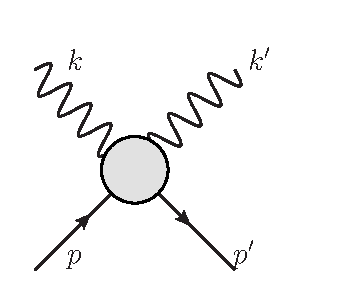
\includegraphics[scale=0.5]{eps/2photon-blob} 
\end{minipage}
$	=	\hspace{1em} 	 $
$\underbrace{ \begin{minipage}{1.3in}
  \begin{center} 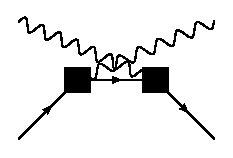
\includegraphics[scale=0.9]{eps/Tree-crossed-square} \end{center}
\end{minipage}}_I$
$\hspace{1em}   +  \hspace{1em} $
$\underbrace{\begin{minipage}{1.3in}
   \begin{center} 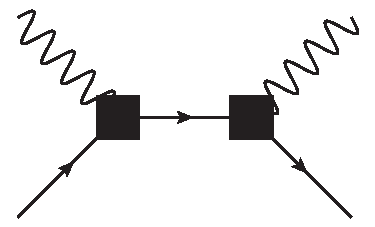
\includegraphics[scale=0.5]{eps/Tree-uncrossed-square} \end{center} 
\end{minipage}}_{II}$
$\hspace{1em}   +  \hspace{1em} $
$\underbrace{\begin{minipage}{1.3in}
   \begin{center} 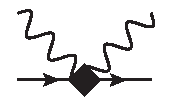
\includegraphics[scale=0.8]{eps/two-photon-nrqed} \end{center} 
\end{minipage}}_{III}$

\vspace{1em}



In each set of diagrams, the vertices represent the \emph{total} electron vertex.  For QED this is determined, as before, by the form factors, and for NRQED it is determined by the calculations of the previous section.

Since the two amplitudes must be equal, in principle the process is this: First calculate the scattering amplitude in QED.  Then, calculate the contribution to the scattering amplitude coming from the tree diagrams I and II above.  Whatever discrepancy remains must be the value of the local two-photon vertex III.   

The process of subtracting the one set of diagrams from the other could be slightly complicated, but luckily it turns out there is a simpler path.  By considering the physical origin of the local terms in NRQED, it will be possible to split the QED diagrams into local and non-local parts, where the latter can be shown to be equal to the non-local diagrams in NRQED.  Then, comparing the two scattering processes becomes much easier.

\subsubsection{Z diagrams}
The high energy theory (QED) doesn't contain any two-photon vertices, while the low energy theory (NRQED) does.  This is a general feature of effective field theories, that new types of local interactions arise.  The high energy theory can have intermediate states that are highly virtual, while the low energy theory doesn't.  Instead, as according to the uncertainty principle, intermediate states with extremely high energy can be considered to occur almost instantaneously, giving rise in the effective theory to local interactions.

How does the local two-photon interaction arise in NRQED?  Of course there are an infinite number of contributions, but we'll consider just the leading order contributions.  These will come from the tree level two photon diagrams as shown above.  Compare the tree-level diagrams in the two theories: in addition to the vertices being different, so are the propagators.  The propagator in QED represents some admixture of the electron and positron field, while in NRQED it is only the electron.
%%%%%%%%
In both QED and NRQED, a process is calculated as the sum of a series of diagrams, representing an expansion in perturbation theory.  However, there is a difference between the two in the nature of perturbation theory employed.

In QED, at each vertex both energy and momentum is conserved.  But intermediate particles may be off mass-shell; that is, it is no longer the case that for a particle of four-momentum $p$ and mass $m$ that $p^2 = m^2$.

In NRQED, the old Rayleigh-Schrodinger perturbation theory is used.   All intermediate particles are on mass-shell.  But at the vertices (when represented diagrammatically), although momenta is conserved, energy is not.  


Remember that in old perturbation theory, corrections have the rough form
\beq
	\Delta =  \Sigma_\text{int} \frac{  \matrixel{\text{out} }{V}{\text{int}} \matrixel{\text{int} }{V}{\text{in}} }{E_\text{in} - E_\text{int}}
	%\Delta = \frac{  \matrixel{A}{B}{C} }{E - E}
\eeq
where the sum is over intermediate states, which can have differing energy from the initial state.

The trick, then, is to take the relativistic tree-level diagrams of QED and rewrite them in the language of  Rayleigh-Schrodinger before trying to compare them to NRQED.  In NRQED, only intermediate states involving electrons can be considered, but in QED intermediate states identified with positrons will appear as well.  It is \emph{these} processes, involving a large violation of energy conservation, that will appear as contact terms in NRQED.  

There are two diagrams in QED, and both can be dealt with in the same general way.  Consider the uncrossed diagram:

%TODO fix diagrams


\vspace{1em}
 \mbox{
\begin{minipage}{1in}
   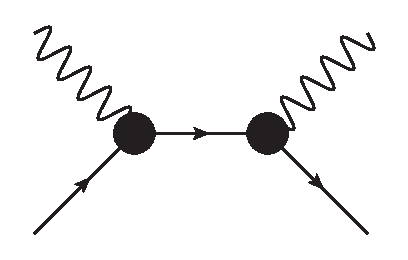
\includegraphics[scale=0.5]{eps/Tree-uncrossed} 
\end{minipage}
$	 \hspace{1em} =	\hspace{1em}	 $
\begin{minipage}{1.5in}
   \begin{center} 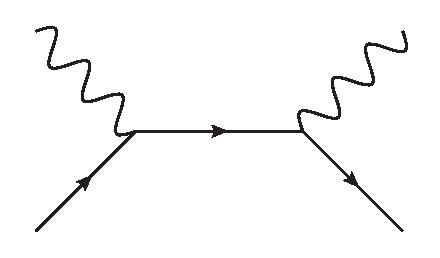
\includegraphics[scale=0.5]{eps/PlainTree} \end{center}
\end{minipage}
$\hspace{1em}   +  \hspace{1em} $
\begin{minipage}{1.5in}
   \begin{center}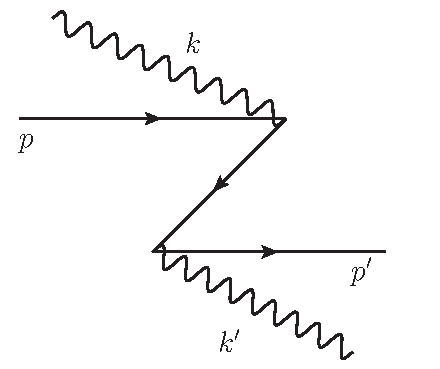
\includegraphics[scale=0.5]{eps/Zdiag} \end{center}
\end{minipage}
} 
\vspace{1em}



There are two tree level processes that can be considered in the old time-ordered perturbation theory.  The first corresponds to an incoming electron, which first absorbs a photon and then emits one.  The second, more complicated process, involves the creation of intermediate positron.  While a free electron travels along, an incoming photon decays into an electron and positron.  Then, the positron annihilates the incoming electron and emits the outgoing photon.  Because of the shape of this diagram, it is called a ``Z diagram.''

In the Z-diagrams, the electrons and the photons are external, so the sum over the intermediate states is specifically the intermediate states of the positrons.  Likewise, the other diagrams are written as a sum over intermediate electron states.  But because of the rules of Rayleigh-Schrodinger perturbation theory, all these states are on mass shell.  And since the momenta here is fixed, the sum over intermediate states is a sum over spin states.

So the original QED diagram should somehow split into two terms, one involving a sum over electron states and the other a sum over anti-particles.  

%TODO insert diagram
Call the intermediate momentum $\v{q}$.  The initial energy will be $q_0$, the intermediate energy will be that of the on mass shell particle, $E_q = \sqrt{\v{q}^2 + m^2 }$.


\vspace{1em}
 \mbox{
\begin{minipage}{1in}
   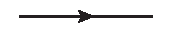
\includegraphics[scale=0.8]{eps/prop} 
\end{minipage}
$	=$ \hspace{1em} $	i\frac{ \cancel{q} -m}{q^2 - m^2}  
		= i\frac{1}{\sqrt{\v{q}^2 + m^2} } \left(
			\frac{ \Sigma u(\v{q}) \bar{u}(\v{q})  }  {q_0 - \sqrt{\v{q}^2 + m^2} }
			+ \frac{ \Sigma v(-\v{q}) \bar{v}(-\v{q})  }  {q_0 + \sqrt{\v{q}^2 + m^2} }
		\right )	 $
} 
\vspace{1em}




This identity can be technically reproduced as follows.  First write the denominator of the propagator as
\beq
	i\frac{ \cancel{q} -m}{q^2 - m^2}   = i \frac{ \cancel{q} -m}{q_0^2 -(\v{q}^2 + m^2)}
\eeq
This could be factored into 
\beq
	q_0^2 -(\v{q}^2 + m^2) = (q_0 + \sqrt{\v{q}^2 + m^2})  (q_0 - \sqrt{\v{q}^2 + m^2})
\eeq
So it implies poles at $q_0 = \pm  \sqrt{\v{q}^2 + m^2}$.  There is one unique way of factoring the original propagator into the two poles:
\beq
	\frac{1}{2\sqrt{\v{q}^2 + m^2}}
		\left(
			\frac{ \gamma^0 \sqrt{\v{q}^2 + m^2} - \v{\gamma} \cdot \v{q} + m}{q_0 - \sqrt{\v{q}^2 + m^2}}
			- \frac{ \gamma^0 \sqrt{\v{q}^2 + m^2} + \v{\gamma} \cdot \v{q} - m}{q_0 + \sqrt{\v{q}^2 + m^2}}
		\right)
\eeq
The two numerators can be exactly equated to sums over polarisation states of electron and positron spinors:
\beqa
	\Sigma u(\v{p}) \bar{u}(\v{p}) &=& \gamma \cdot p + m	\\
	\Sigma v(\v{p}) \bar{v}(\v{p}) &=& \gamma \cdot p - m	
\eeqa
These relations hold for particles which are on mass-shell.  That is exactly the case here.  But then, there is an assumption that the quantity $p_0$ above is the on mass-shell energy, $\sqrt{\v{p}^2 + m^2}$.

So, noting that particles with momentum $\pm \v{q}$ have the same energy $\sqrt{\v{q}^2 + m^2}$ and that $q_0$ is the off-mass shell energy from the relativistic diagram, the propagator can be rewritten:
\beq
	\frac{1}{2\sqrt{\v{q}^2 + m^2}}
		\left(
			\frac{\Sigma u(\v{q}) \bar{u}(\v{q}) }{q_0 - \sqrt{\v{q}^2 + m^2}}
			- \frac{  \Sigma v(-\v{q}) \bar{v}(-\v{q})}{q_0 + \sqrt{\v{q}^2 + m^2}}
		\right)
\eeq
The numerators have now been put into exactly the forms expected for the regular- and Z-diagrams of old perturbation theory. 


As mentioned above this can be understood in the context of old perturbation theory as sum over intermediate states in the numerator,  with the expected form of the denominator being $E_\text{in} - E_\text{int}$.  It can be shown that the denominators have exactly this form. 

Now consider the first, regular diagram.  The initial energy is $q_0$, since in relativistic theory the total energy at the vertex is conserved.  The intermediate energy is the on-mass shell energy of the electron: $\sqrt{\v{q}^2+ m^2}$.  Thus the denominator of $q_0 - \sqrt{\v{q}^2+ m^2}$ is as expected.

Now consider the Z-diagram.  The initial energy is still $q_0$.  The intermediate energy is more complicated: there are two photons, two electrons, and a positron present.  The total combined energy is:
\beq
	E_\text{int} = p_0 + p'_0 + k_0 + k'_0 + \sqrt{\v{q}^2 + m^2} = 2q_0 +  \sqrt{\v{q}^2 + m^2}
\eeq
Then the difference $E_\text{in} - E_\text{int} = -q_0 - \sqrt{\v{q}^2 + m^2}$, as expected.

So rewriting the propagator into these two separate terms can be understood as how the fully relativistic process appears in old perturbation theory.  In a relativistic theory, intermediate states involving positrons must be accounted for.  For higher order QED diagrams more complicated processes will appear, but at the tree level only those discussed above are involved.  No approximations are involved --- the identity for the propagator is exact.  The form is more convenient for discussing nonrelativistic energies, but is still equivalent to the relativistic diagrams.

%Four equations for each of the diagrams





\subsubsection{Relation between NRQED and old perturbation theory}
Now it is necessary to show how the diagrams in old perturbation theory relate to those of NRQED.  

The normal diagrams can be easily interpreted as the product of vertices and the relativistic Rayleigh-Schrodinger propagator:
%Equation with diagram on left, prodcut of verices on right

\vspace{1em}
 \mbox{
\begin{minipage}{1.6in}
   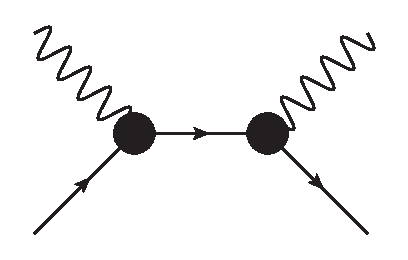
\includegraphics[scale=0.5]{eps/Tree-uncrossed} 
\end{minipage}
$	=	\hspace{2em} 	\Bigg( $
\begin{minipage}{0.8in}
  \begin{center} 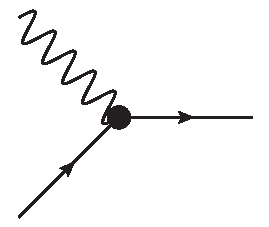
\includegraphics[scale=0.4]{eps/vertex-in} \end{center}
\end{minipage}
$\Bigg ) \times \Bigg ($
\begin{minipage}{0.6in}
   \begin{center} 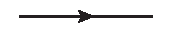
\includegraphics[scale=0.5]{eps/prop} \end{center} 
\end{minipage}
$\Bigg ) \times \Bigg ($\begin{minipage}{0.8in}
   \begin{center} 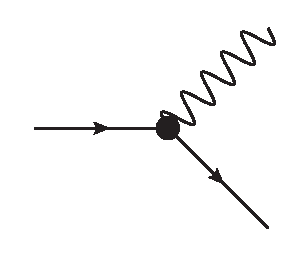
\includegraphics[scale=0.4]{eps/vertex-out} \end{center} 
\end{minipage}
$\Bigg )$
} 
\vspace{1em}
 




%Define each piece
%Vertex in, prop, vertex out
Recall that the total NRQED one-photon vertex was derived by comparing to the QED vertex, so necessarily
\beq
	\bar{u} \Gamma^0 u = \phi^\dagger V^0 \phi , \;  \bar{u} \Gamma^i u = \phi^\dagger V^i \phi
\eeq 
The propagator $1/(q_0 - \sqrt{m^2 + \v{q}^2})$ is equal to the total propagator in NRQED (including relativistic corrections).  So it really is the case that the two sets of diagrams are equivalent.  Whether the vertices are written in terms of NRQED or QED, the ultimate expression will be the same.

It then follows that the contributions to the local contact term in NRQED come (at tree level) exactly from the Z-diagrams.  To calculate the contact terms to the order (in the nonrelativistic expansion) needed, the Z-diagrams need to be approximated just as the one-photon vertex diagrams were in the previous section.  Then the NRQED coefficients can be obtained by comparing the two calculations.  

At nonrelativistic energies, it would be expected that the sum over intermediate states now does not resemble a propagator.  Because only terms involving up to one power of momentum need be kept, the square root term becomes simply $m$.  $q_0$, the total incoming energy, will involve both the electron and photon energy.  Depending on whether the crossed or uncrossed diagram is considered, it will be either $q_0 = p_0 + k_0$ or $q_0 = p_0 - k'_0$.  In either case, it will be $m$ at the leading order, with a first order correction due to the photon energy. 
\beq
	\frac{ \Sigma \bar{v}(-\v{q}) v(-\v{q}) }  {q_0 + \sqrt{\v{q}^2 + m^2} } 
		\approx \frac{ \Sigma \bar{v}(-\v{q}) v(-\v{q}) }  {2m + (q_0-m) }
\eeq
Since $q_0-m << m$, this can then be written as 
\beq
		\approx  \left( 1 - \frac{q_0-m}{2m} \right ) \frac{ \Sigma \bar{v}(-\v{q}) v(-\v{q}) }  {2m}
\eeq
In this approximation, the two Z diagrams become


\vspace{1em}
 \mbox{
\begin{minipage}{1.2in}
   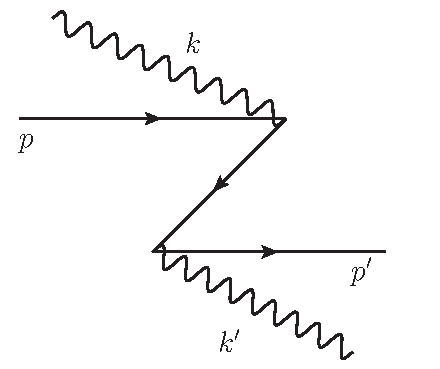
\includegraphics[scale=0.4]{eps/Zdiag} 
\end{minipage}
= \hspace{1em}
\small$	
\Sigma_{\text{spin}}
\left( 1 - \frac{k_0}{2m} \right ) \frac{1}{2m} 
	\bar{u}(\v{p'}) \gamma^\mu \epsilon^*_\mu(k') v_s(-\v{p} - \v{k}) \bar{v}_s(-\v{p} - \v{k}) \Gamma^\nu \epsilon_\nu(k) u(\v{p})
$\normalsize
} 
\vspace{1em}


\vspace{1em}
 \mbox{
\begin{minipage}{1.2in}
   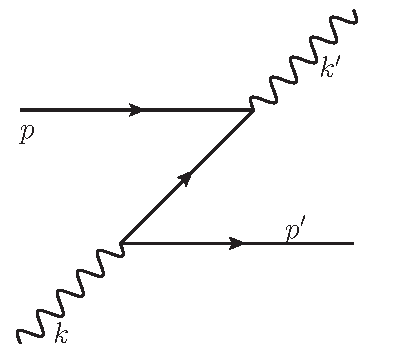
\includegraphics[scale=0.4]{eps/Zdiag2} 
\end{minipage}
= \hspace{1em}
\small $	
\Sigma_{\text{spin}}
\left( 1 + \frac{k'_0}{2m} \right ) \frac{1}{2m} 
	\bar{u}(\v{p'}) \gamma^\mu \epsilon_\mu(k) v(\v{k'} - \v{p})_s \bar{v}_s(\v{k'} - \v{p}) \Gamma^\nu \epsilon^*_\nu(k') u(\v{p})
$ \normalsize
} 
\vspace{1em}

While the sums over intermediate states could also be expanded, it'll be easiest to calculate these in the above form.  The vertices will be the sum of particle-antiparticle bilinears, which can be calculated separately.



\subsection{Nonrelativistic expressions for Z diagrams}


Looking at the equations for the Z diagrams, they are both the product of two types of terms to calculate:

\beq \label{eq:Sh:uvGamma}
	\bar{u}(\v{p'}) \Gamma^\mu(q) v(\gv{\ell}) \;  \text{and} \; \bar{u}(\gv{\ell}) \Gamma^\mu(q) v(\v{p})
\eeq
Here $\ell$ is the intermediate momentum of the positron, and $q$ is the momentum of the photon going into the vertex (either $k$ or $-k'$).  The form of $\Gamma$ is
\beq
	\Gamma^\mu(q) = F_1 \gamma^\mu + F_2 \frac{q_\nu \sigma^{\mu\nu}}{2m}
\eeq
To compare the Z diagrams to the contact terms of NRQED, first express the bilinears in the vertices of \eqref{eq:Sh:uvGamma} in terms of the nonrelativistic quantities.  This can be done for each of the two terms in $\Gamma^\mu$ separately.  The bispinors $u$ will be replaced by the spinor $\phi$, as before.  Now, the bispinor $v$ will be replaced by a spinor for a positron, which shall be called $\chi$.  In doing the expansion only terms up to $\mathcal{O}(1/m)$ need be kept.


To calculate the vector like bilinears, treat the spatial and time-like components separately.  First $\mu=0$:
\beqa
	\ubar(p') \gamma^0 v(\ell)
		&=&	\udaggervec{\v{p'}} \vvec{\v{q}}	\\
		&=&	\phi^\dagger \left( \frac{ \sigdot{\ell} + \sigdot{p'} }{2m} \right ) \chi	\\
	\vbar{\ell} \gamma^0 u(p)
		&=&	\vdaggervec{\ell} \uvec{p}	\\
		&=&	\chi^\dagger \left( \frac{ \sigdot{\ell} + \sigdot{p} }{2m} \right ) \phi	
\eeqa
Then $\mu=i$:
\beqa
	\ubar(p') \gamma^i v(\ell)
		&=&	\udaggervec{p'} \begin{pmatrix} 0 & \sigma_i \\ \sigma_i & 0 \end{pmatrix} \vvec{\ell}	\\
		&=&	\phi^\dagger \sigma_i \chi \\
	\vbar(\ell) \gamma^i u(p)
		&=&	\vdaggervec{\ell} \begin{pmatrix} 0 & \sigma_i \\ \sigma_i & 0 \end{pmatrix} \uvec{p}	\\
		&=&	\chi^\dagger \sigma_i \phi 
\eeqa

In the tensor terms a factor of momentum $q_\nu$ appears.  The spatial part, $q_j$ is ``naturally raised" so $q_j = -(\v{q})_j$.  As before the two types of indices should be treated separately.  For $\mu=0$:

\beqa
	\frac{i q_\nu}{2m} \ubar(p') \sigma^{0 \nu} v(\ell) 
		&=& \frac{i q_j}{2m} \ubar(p') \sigma^{0j} v(\ell) \\
		&=& -\frac{q_j}{2m} \udaggervec{p'} \Mblock{0}{\sigma^i}{-\sigma^i}{0} \vvec{\ell}	\\
		&=& \phi^\dagger \frac{ \sigdot{q}}{2m} \chi	\\
	\frac{i q_\nu}{2m} \vbar(\ell) \sigma^{0 \nu} u(p) 
		&=& \frac{i q_j}{2m} \vbar(\ell) \sigma^{0j} u(p) \\
		&=& -\frac{q_j}{2m} \vbar{\ell} \Mblock{0}{\sigma^i}{-\sigma^i}{0} \uvec{p}	\\
		&=& -\chi^\dagger \frac{ \sigdot{q}}{2m} \phi	\\
\eeqa
Then for $\mu=i$
\beq
	\frac{i q_\nu}{2m} \ubar(p') \sigma^{i \nu} v(\ell)
	 	= \frac{i q_0}{2m} \ubar(p') \sigma^{i 0} v(\ell) + \frac{i q_j}{2m} \ubar(p') \sigma^{i j} v(\ell)	
\eeq
\beq
	 = - \frac{i q_0}{2m}  \udaggervec{p'} \Mblock{0}{\sigma^i}{-\sigma^i}{0} \vvec{\ell} 	
	 	+ \frac{i q_j}{2m}  \epsilon_{ijk}  \udaggervec{p'} \Mblock{\sigma^k}{0}{0}{\sigma^k} \vvec{\ell} \nonumber
\eeq
The second term will be of order $\mathcal{O}(1/m^2)$ and so can be neglected.  So 
\beq
	\frac{i q_\nu}{2m} \ubar(p') \sigma^{i \nu} v(\ell) 
		= \phi^\dagger \frac{q_0 \sigma_i}{2m} \chi
\eeq
The complementary term is 
\beq
	\frac{i q_\nu}{2m} \vbar(\ell) \sigma^{i \nu} u(p)
	 	= \frac{i q_0}{2m} \vbar(\ell) \sigma^{i 0} v(\ell) + \frac{i q_j}{2m} \ubar(p') \sigma^{i j} u(p)	
\eeq
Again,  the second term with $\sigma^{ij}$ has the same general structure and will be of order $1/m^2$.  So 
\beqa
		\frac{i q_\nu}{2m} \vbar(\ell) \sigma^{i \nu} u(p)
	 &=&	\frac{i q_0}{2m} \vdaggervec{\ell} \Mblock{0}{\sigma^i}{-\sigma^i}{0} \uvec{p} 	\\
	 &=&	- \chi^\dagger \frac{q _0 \sigma^i}{2m} \phi
\eeqa

Now the total vertices $\ubar \Gamma^\mu v$ can be expressed nonrelativistically:

\beq
	\ubar(p') \Gamma^0 v(\ell)  
		=  \phi^\dagger(p') \left( F_1 \frac{ \sigdotg{\ell} + \sigdot{p'} }{2m} + F_2 \frac{ \sigdot{q} } {2m} \right ) \chi(\ell)
\eeq

\beq
	\vbar(\ell) \Gamma^0 v(p)  
		=  \chi^\dagger(p') \left( F_1 \frac{ \sigdotg{\ell} + \sigdot{p} }{2m} + F_2 \frac{ \sigdot{q} } {2m} \right ) \phi(\ell)
\eeq
	
\beq
	\ubar(p') \Gamma^i v(\ell)  
		= \phi^\dagger \left( F_1 + F_2 \frac{q_0}{2m} \right) \sigma^i \chi
\eeq
			
\beq
	\vbar(\ell) \Gamma^i v(p)  
		= \chi^\dagger \left( F_1 - F_2 \frac{q_0}{2m} \right) \sigma^i \phi
\eeq			

Returning to the Z diagrams, the structures $\Gamma^\mu$ appear contracted with the photon polarization.  Because a physical process is being calculated, the result should not depend on the gauge chosen.  So it will be easiest to choose the gauge where the photons are transverse and $\epsilon_0 = 0$.  Then $\Gamma \cdot \epsilon = - \gv{\Gamma} \cdot \gv{\epsilon}$.

\vspace{1em}
 \mbox{
\begin{minipage}{1in}
   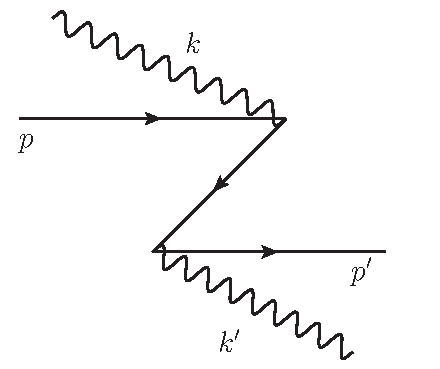
\includegraphics[scale=0.4]{eps/Zdiag} 
\end{minipage}
 = \hspace{0.5em}
\begin{minipage}{3in}
\beq
\begin{split}
	\Sigma_{\text{spin}}
	\left( 1 - \frac{k_0}{2m} \right ) &\frac{1}{2m} 
		\left[ \phi^\dagger \left( F_1 + F_2 \frac{ -k'_0}{2m} \right ) \gv{\sigma} \cdot \gv{\epsilon}^*(k') \chi \right]
\\ &	\times	\left[ \epsilon_j(k) \chi^\dagger \left( F_1 - F_2 \frac{k_0}{2m} \right)  \gv{\sigma} \cdot  \gv{\epsilon}(k)   \phi \right ]	
\end{split}
\eeq
\end{minipage}
} 
\vspace{1em}

The sum over intermediate spin spates just becomes the identity: $\Sigma_{\text{spin}} \chi^\dagger \chi = 1$. 
\beq
	= \frac{1}{2m} \left( 1 - \frac{k_0}{2m} \right ) \phi^\dagger \left[ 
			\left( F_1 - F_2 \frac{k'_0}{2m} \right )
			\left( F_1 - F_2 \frac{k_0}{2m} \right)
			\gv{\sigma} \cdot \gv{\epsilon}^*(k')  \gv{\sigma} \cdot  \gv{\epsilon}(k)  
		\right ] \phi
\eeq
	
Since only terms up to order $1/m$ are needed, this can be simplified.  Also, in this approximation $k'_0 \approx k_0$, as the total conservation of energy implies $k'_0 - k_0 = p_0 - p'_0 \sim \v{p}^2/m^2$.  So for convenience everything will be written in terms of $k_0$.  

\beq
	= \frac{1}{2m}  \phi^\dagger \left[ 
			\left( F_1^2 - F_1 [F_1 + 2 F_2 ] \frac{k_0}{2m} \right )
			\gv{\sigma} \cdot \gv{\epsilon}^*(k')  \gv{\sigma} \cdot  \gv{\epsilon}(k)  
		\right ] \phi
\eeq


The other Z diagram, coming from the crossed diagram is:

\vspace{1em}
 \mbox{
\begin{minipage}{1in}
   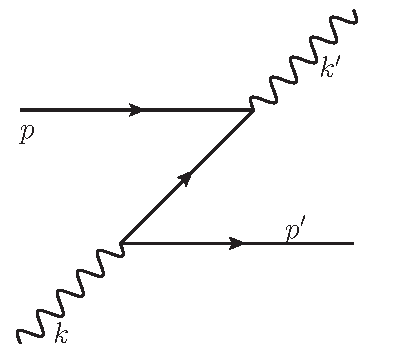
\includegraphics[scale=0.4]{eps/Zdiag2} 
\end{minipage}
= \hspace{0.5em}
\scriptsize$	
\Sigma_{\text{spin}}
\left( 1 + \frac{k'_0}{2m} \right ) \frac{1}{2m} 
	\left[ \phi^\dagger \left( F_1 + F_2 \frac{ k_0}{2m} \right ) \gv{\sigma} \cdot \gv{\epsilon}^(k) \chi \right]
	\left[ \epsilon_j(k) \chi^\dagger \left( F_1 + F_2 \frac{k'_0}{2m} \right)  \gv{\sigma} \cdot  \gv{\epsilon}^*(k')   \phi \right ]	
$\normalsize
} 
\vspace{1em}

After summing over spin states this becomes
\beq
	 \frac{1}{2m} \left( 1 + \frac{k'_0}{2m} \right ) \phi^\dagger \left[ 
			\left( F_1 + F_2 \frac{k_0}{2m} \right )
			\left( F_1 + F_2 \frac{k'_0}{2m} \right)
			\gv{\sigma} \cdot \gv{\epsilon}^(k)  \gv{\sigma} \cdot  \gv{\epsilon}^*(k')  
		\right ] \phi.
\eeq
And then applying the same simplifications as before results in
\beq
	 \frac{1}{2m}  \phi^\dagger \left[ 
			\left( F_1^2 + F_1 [F_1 + 2 F_2 ] \frac{k_0}{2m} \right )
			\gv{\sigma} \cdot \gv{\epsilon}^(k)  \gv{\sigma} \cdot  \gv{\epsilon}^*(k')  
		\right ] \phi.
\eeq

The local interaction comes from the sum of the two diagrams.  Adding them together,

%TODO add diagram?
\mbox{
\begin{minipage}{0.6in}
   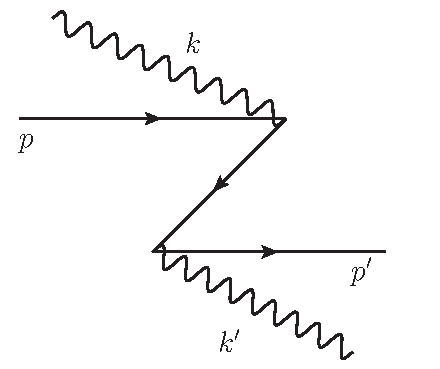
\includegraphics[scale=0.2]{eps/Zdiag} 
\end{minipage}
+
\begin{minipage}{0.6in}
   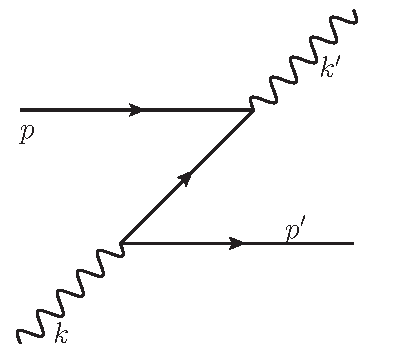
\includegraphics[scale=0.2]{eps/Zdiag2} 
\end{minipage}
\begin{minipage}{2in}
\begin{equation*}
=
\begin{split}
 & \frac{1}{2m} \phi^\dagger \Bigg [
	 \left( F_1^2 + F_1 [F_1 + 2 F_2 ] \frac{k_0}{2m} \right )
			\gv{\sigma} \cdot \gv{\epsilon}^(k)  \gv{\sigma} \cdot  \gv{\epsilon}^*(k')  \\
	&+ 
			\left( F_1^2 - F_1 [F_1 + 2 F_2 ] \frac{k_0}{2m} \right )
			\gv{\sigma} \cdot \gv{\epsilon}^*(k')  \gv{\sigma} \cdot  \gv{\epsilon}(k)  
		 \Bigg ] \phi	
\end{split}
\end{equation*}
\end{minipage}
}
\beq
\begin{split}
=&
		\frac{F_1}{2m}  \phi^\dagger \Bigg [
			F_1 \{ \gv{\sigma} \cdot \gv{\epsilon},   \gv{\sigma} \cdot  \gv{\epsilon}^* \}
			+ (F_1 + 2F_2) \frac{k_0}{2m} [ \gv{\sigma} \cdot \gv{\epsilon},   \gv{\sigma} \cdot  \gv{\epsilon}^* ]
		 \Bigg ] \phi	\\
	=&
		\frac{F_1}{m}  \phi^\dagger \Bigg [
			F_1  \gv{\epsilon} \cdot  \gv{\epsilon}^* 
			+ (F_1 + 2F_2) \frac{k_0}{2m} \gv{\sigma} \cdot \gv{\epsilon} \times  \gv{\epsilon}^* 
		 \Bigg ] \phi
\end{split}
\eeq
It now remains to calculate the same amplitude in NRQED and compare.
		
\subsection{Compton scattering in NRQED}
The idea is to calculate the Compton scattering in the nonrelativistic theory.  The gauge is chosen such that the photon polarisations obey $\epsilon_0 = 0$.  In general, both terms arising from two-photon vertices, and those from tree level diagrams of two one-photon vertices, should be considered.  However, because of the approach taken in calculating the process from the relativistic Lagrangian, only the former terms are needed.  That is, contact terms (which arise from some combination of Z-diagrams in the relativistic theory)  are separated from the rest.  

Further, ultimately only a few of these terms are relevant -- terms which have both $\v{B}$ and $\v{A}$ can be ignored.

The remaining terms of interest are:
\scriptsize
\beqa
	\mathcal{L}_{A^2} &=& \fnr^\dagger ( - \frac{e^2 \v{A}^2}{2m}  - e^2 \frac{ \{ \grad^2, \v{A}^2 \} 
}{8m^3} - e^2\frac{ \{\nabla_i, A_i \} \{\nabla_j, A_j\} }{8m^3}
		+ c^2_S \frac{ e^2 \v{S} \smalldot ( \v{A} \times \v{E} - \v{E} \times \v{A} )}{8m^2} ) \fnr
\eeqa
\normalsize

The process considered has an incoming photon with momentum $k$ and polarisation $\epsilon(k)$, and an outgoing photon with momentum $k'$ and polarisation $\epsilon^*(k')$.  The charged particle has incoming momentum $p$ and outgoing $p'= p + k - k'$.

As in the single-photon calculation, it is simply a matter of reading terms off the Lagrangian.  To find the scattering amplitude,  replace $\Psi$ with $\phis$, and replace $\v{A}$ with photon polarisations $\epsilon$ and $\epsilon^*$.  In the gauge chosen, $\v{E}(k) = -\partial_0 \v{\A} = i k_0 \gv{\epsilon}(k) = -ik'_0 \gv{\epsilon^*}(k') $ .

Contracted with the photon of momentum $k$, the result is $\v{E} \to i k_0 \v{\A}$, while with the photon of momentum $k'$ it is $\v{E} \to i k'_0 \v{\Adag}$.  Both processes must be considered in calculating the scattering, so:
\[
	\v{A} \times \v{E} = - \v{A} \times (\partial_0 \v{A})
		\to 
	-i(k_0' \v{\epsilon} \times \v{\epsilon} - k_0 \v{\epsilon} \times \v{\epsilon} ) = i ( k_0' + k_0) \v{\epsilon} \times \v{\epsilon}^*
\]
And
\[
	\v{E} \times \v{A} = - (\partial_0 \v{A}) \times  \v{A}
		\to 
	-i( k_0 \v{\epsilon} \times \v{\epsilon^*} - k_0' \v{\epsilon^*} \times \v{\epsilon} ) = -i ( k_0' + k_0) \v{\epsilon} \times \v{\epsilon^*}
\]
So from the term in the Lagrangian 
\[
 c_S \Psi^\dagger \frac{ e^2 \v{S} \smalldot ( \v{A} \times \v{E} - \v{E} \times \v{A} )}{8m^2} ) \Psi
\]
appears in the scattering amplitude
\[
  -i c_S \phi^\dagger  \Big ( \frac{e^2}{4m^2}    i(k_0 + k_0')    \v{\epsilon} \times \v{\epsilon^*} \Big ) \phi
	=
     c_S \frac{e^2}{4m^2} \phi^\dagger  \Big ( (k_0 + k_0')    \v{\epsilon} \times \v{\epsilon^*} \Big ) \phi
\]
Using the approximation $k_0 \approx k'_0$, that part of the amplitude now becomes
\beq \label{eq:Sh:ComptNR}
     c_S \frac{e^2}{2m^2} \phi^\dagger  \Big ( k_0    \v{\epsilon} \times \v{\epsilon^*} \Big ) \phi
\eeq


This is the part of the amplitude wanted to compare for reasons of consistency.
	

\subsection{Comparison of QED and NRQED Compton scattering}
Now that the amplitude has been calculated in both theories, the coefficient of NRQED $c_S$ can be fixed.  Using that $F_1 = e$ and $F_2 = e\frac{g-2}{2}$, $F_1 + 2F_2 = e^2(g-1)$.
So the final result is that 
\beq
	c_S = g-1
\eeq
 



